\documentclass[12pt]{article}

\usepackage{ishn}

\makeindex[intoc]

\begin{document}

\hypersetup{pageanchor=false}
\begin{titlepage}
	\begin{center}
		\vspace*{1em}
		\Huge
		\textbf{III Quantum Field Theory}

		\vspace{1em}
		\large
		Ishan Nath, Michaelmas 2024

		\vspace{1.5em}

		\Large

		Based on Lectures by Prof. Alejandra Castro

		\vspace{1em}

		\large
		\today
	\end{center}
	
\end{titlepage}
\hypersetup{pageanchor=true}

\tableofcontents

\newpage

% lecture 1

\setcounter{section}{-1}

\section{Introduction}%
\label{sec:intro}

We are following Tong's notes mostly, and Matt Schwartz book for a part of it.

Our goal is to combine quantum mechanics and special relativity. The result is that the number of particles is not preserved.

Key points of this theory is that it is robust and systematic, and governed by a few principles:
\begin{itemize}
	\item locality,
	\item symmetries,
	\item renormalization.
\end{itemize}

There are some units and conventions we will need. In terms of the base units $L, T, M$ (length, time and mass), then
\begin{align*}
	[c] &= [LT^{-1}], \\
	[\hbar] &= [L^2 M T^{-1}], \\
	[G] &= [L^3M^{-1}T^{-2}].
\end{align*}
We take natural units, so $c = 1 = \hbar$, meaning $L = T = M^{-1}$. We refer to the mass dimension of quantities, so $[G] = [M^{-2}] = -2$. Note $M$ also has dimensions of energy.

We will be using the relativistic notation
\[
\eta^{\mu\nu} =
\begin{pmatrix}
	1 & & & \\ & -1 & & \\ & & -1 & \\ & & & -1
\end{pmatrix}.
\]
When talking about spacetime, we let $X^\mu = (t, x, y, z)$.

\newpage

\section{Classical Field Theory}%
\label{sec:classical_ft}

In classical mechanics, a natural object is the action
\[
	S(t_1, t_2) = \int_{t_1}^{t_2} \diff t \, \left( m \sum_{i = 1}^3 \left( \frac{\diff x_i}{\diff t} \right)^2 - V(X^\mu) \right).
\]
Some basic facts of the action is that:
\begin{enumerate}
	\item Equations of motion are given by extremizing $S$.
	\item Boundary conditions are supplied externally.
	\item $S$ is built on symmetries of the system.
\end{enumerate}

We declare in field theory that the fundamental object is a \emph{field}:
\[
	\phi_a(t, \mathbf{x}) : \mathbb{R}^{3, 1} \to \mathbb{R} \text{ or } \mathbb{C} \text{ or } \mathbb{R}^n.
\]
Here $a$ denotes the type of the field. The first consequence is that we are dealing with an infinite number of degrees of freedom.

\begin{exbox}[Electromagnetism]
	In EM, the \emph{gauge field} is
	\[
	A^\mu(x) = (\phi(x), \mathbf{A}(x)).
	\]
	The Maxwell equations are
	\begin{align*}
		\mathbf{E} &= - \nabla \phi - \frac{\partial \mathbf{A}}{\partial t} & \nabla \cdot \mathbf{E} &= \rho, \\
		\mathbf{B} &= \nabla \cdot \mathbf{A}, & \nabla \times \mathbf{B} &= \mathbf{J} + \frac{\partial \mathbf{E}}{\partial t}.
	\end{align*}
	We have two identities:
	\[
	\nabla \cdot \mathbf{B} = 0, \qquad \frac{\diff \mathbf{B}}{\diff t} = \nabla \times \mathbf{E}.
	\]
\end{exbox}

\subsection{Lagrangians}%
\label{sub:lag}

Recall the \emph{Lagrangian} is $L = T - V$, and the action can be written
\[
S = \int \diff t \, L.
\]
We can write
\[
L = \int \Diff3 x \, \mathcal{L}(\phi_a, \partial_\mu \phi_a),
\]
for $\mathcal{L}$ the \emph{Lagrangian density} (or just Lagrangian). Then
\[
S = \int \diff t\, L = \int \Diff4 x \, \mathcal{L}.
\]
The equations of motion can be determined by extremizing over fields. One crucial assumption is that $\mathcal{L}$ depends on $\phi_a$ and $\partial_\mu \phi_a$, and not any higher derivatives. Then,
\begin{align*}
	\delta S &= \int \Diff4 x \left[ \frac{\partial \mathcal{L}}{\partial \phi_a} \delta \phi_a + \frac{\partial \mathcal{L}}{\partial(\partial_\mu \phi_\alpha)} \delta(\partial_\mu \phi_a) \right] \\
		 &= \int \Diff4 x \left[ \frac{\partial \mathcal{L}}{\partial \phi_a} \delta \phi_a - \partial_\mu \left( \frac{\partial \mathcal{L}}{\partial(\partial_\mu \phi_a)} \right) \delta \phi_a + \partial_\mu \left( \frac{\partial \mathcal{L}}{\partial (\partial_\mu \phi_a)} \delta \phi_a \right) \right].
\end{align*}
The last term is a total derivative, and if we assume that fields decay at infinity this evaluates to $0$. Hence requiring $\delta S = 0$ gives
\[
\partial_\mu \left( \frac{\partial \mathcal{L}}{\partial (\partial _\mu \phi_a)} \right) - \frac{\partial \mathcal{L}}{\partial \phi_a} = 0.
\]
\begin{exbox}[Free massive scalar field]
	The `simplest' Lagrangian is
	\begin{align*}
		\mathcal{L} &= \frac{1}{2} \eta^{\mu\nu} \partial_\mu \phi \partial_\nu \phi - \frac{1}{2} m^2 \phi^2 \\
			    &= \frac{1}{2} \dot \phi^2 - \frac{1}{2} ( \nabla \phi)^2 - \frac{1}{2} m^2 \phi^2.
	\end{align*}
	In traditional classical mechanics, the first term is the kinetic energy, and the other two terms give the potential energy.

	In QFT, kinetic terms are any bilinear terms of the fields. So this Lagrangian is all kinetic terms, and no potential terms.

	The equations of motion in this field are
	\[
	\partial_\mu \partial^\mu \phi + m^2 \phi = \square \phi + m^2 \phi = 0.
	\]
	This is the \emph{Klein-Gordon equation}.
\end{exbox}

% lecture 2

\subsection{Hamiltonians}%
\label{sub:ham}

In this setup, one starts by defining the \emph{canonical momentum}\index{canonical momentum}
\[
\Pi^a(x) = \frac{\partial \mathcal{L}}{\partial(\partial_t \phi_a)} = \frac{\partial \mathcal{L}}{\partial \dot \phi_a}.
\]
The \emph{Hamiltonian density}\index{Hamiltonian density} is
\[
\mathcal{H} = \Pi^a \partial_t \phi_a - \mathcal{L}.
\]
The \emph{Hamiltonian}\index{Hamiltonian} is
\[
H = \int \Diff4 x \, \mathcal{H}.
\]

\begin{exbox}[Scalar field with potential]
	Here our Lagrangian is
	\[
	\mathcal{L} = \frac{1}{2} \eta^{\mu \nu} \partial_\mu \phi \partial_\nu \phi - V(\phi).
	\]
	The canonical momentum is
	\[
	\Pi = \frac{\partial \mathcal{L}}{\partial \dot \phi} = \dot \phi.
	\]
	The Hamiltonian is
	\[
	H = \int \Diff4 x \, (\Pi \partial_t \phi - \mathcal{L}) = \int \Diff4 x \left( \frac{1}{2} \dot \phi^2 + \frac{1}{2} (\nabla \phi)^2  + V(\phi) \right).
	\]
\end{exbox}

\subsection{Symmetries}%
\label{sub:sym}

Symmetries will:
\begin{itemize}
	\item Dictate the actions we write.
	\item Dictate the class of fields (operators) used.
	\item Control the observables we will compute.
\end{itemize}

\subsubsection{Lorentz Invariance}%
\label{subsub:lorentz}

The \emph{Lorentz group}\index{Lorentz group} is defined by
\[
x^\mu \to x'^\mu = \Lambda\indices{^{\mu}_{\nu}} x^\nu,
\]
which preserves the interval
\[
s^2 = x^\mu x^\nu \eta_{\mu\nu} = t^2 - \mathbf{x}^2.
\]
So $s^2 \to s'^2 = s^2$. This condition implies that
\[
\eta_{\mu\nu} \Lambda\indices{^{\mu}_{\rho}} \Lambda\indices{^{\nu}_{\sigma}} = \eta_{\rho\sigma},
\]
or in terms of matrices,
\[
\Lambda^T \eta \Lambda = \eta.
\]

\begin{exbox}
	\begin{enumerate}
		\item Rotations: Say $t' = t$, and $\Lambda\indices{^{i}_{j}} = R\indices{^{i}_{j}}$, for $R \in O(3)$. A rotation in the $x$-$y$ plane is given by
		\[
		\Lambda =
		\begin{pmatrix}
			1 & 0 & 0 & 0 \\
			0 & \cos \theta & - \sin \theta & 0 \\
			0 & \sin \theta & \cos \theta & 0 \\
			0 & 0 & 0 & 1
		\end{pmatrix}.
		\]
	\item Boosts: these mix time and space. A boost in the $(t, x)$ plane is
		\[
		\Lambda =
		\begin{pmatrix}
			\cosh \eta & - \sinh \eta & 0 & 0 \\
			- \sinh \eta & \cosh \eta & 0 & 0 \\
			0 & 0 & 1 & 0 \\
			0 & 0 & 0 & 1
		\end{pmatrix}.
		\]
		Here $\eta$ is the rapidity, and
		\[
			\cosh \eta = \frac{1}{\sqrt{1 - v^2}}, \qquad \sinh \eta = \frac{v}{\sqrt{1 - v^2}}.
		\]
	\end{enumerate}
\end{exbox}

More generally, if we take the determinant of $\Lambda^T \eta \Lambda = \eta$, we find
\[
\det (\Lambda)^2 = 1 \implies \det \Lambda = \pm 1.
\]
If $\det \Lambda = 1$, this is called a \emph{proper Lorentz transformation}\index{Lorentz transformation}. If $\det \Lambda = -1$, this is a \emph{improper Lorentz transformation}.

Proper Lorentz transformations can be continuously connected to the identity, whereas improper Lorentz transformation include symmetries such as parity, and time reversal.

If we focus on $\det \Lambda = 1$, we can then write
\[
\Lambda\indices{^{\mu}_{\nu}} = \delta\indices{^{\mu}_{\nu}} + \eps\indices{^{\mu}_{\nu}} + \mathcal{O}(\eps^2).
\]
What are the properties of $\eps\indices{^{\mu}_{\nu}}$? Plugging this formula into the definition of a Lorentz transformation, we find
\begin{align*}
	\eta_{\rho\sigma} &= \eta_{\mu\nu} (\delta\indices{^{\mu}_{\rho}} + \eps\indices{^{\mu}_{\rho}} + \cdots)(\delta\indices{^{\nu}_{\sigma}} + \eps\indices{^{\nu}_{\sigma}} + \cdots) \\
			  &= \eta_{\mu\nu} \delta\indices{^{\mu}_{\rho}} \delta\indices{^{\nu}_{\sigma}} + \eta_{\mu\nu} \eps\indices{^{\mu}_{\rho}} \delta\indices{^{\nu}_{\sigma}} + \eta_{\mu\nu} \delta\indices{^{\mu}_{\rho}} \eps\indices{^{\nu}_{\sigma}} + \mathcal{O}(\eps^2) \\
			  &= \eta_{\rho\sigma} + \eps_{\sigma\rho} + \eps_{\rho\sigma} + \cdots
\end{align*}
Hence $\eps_{\sigma\rho} = - \eps_{\rho\sigma}$, which gives an anti-symmetric tensor. Therefore, in 3+1 dimensions, we have 6 components. Therefore, we have 6 generators for the Lorentz group, 3 rotations and 3 boosts.

In this context, a field is an object that depends on some coordinates, and has a definite transformation under Lorentz: if $x \to x' = \Lambda x$, then
\[
	\phi_a(x) \to \phi_a'(x) = D[\Lambda]\indices{_{a}^b} \phi_b(\Lambda^{-1}x).
\]
Here $D$ forms a representation of the Lorentz group, so
\begin{itemize}
	\item $D[\Lambda_1] D[\Lambda_2] = D[\Lambda_1 \Lambda_2]$,
	\item $D[\Lambda^{-1}] = D[\Lambda]^{-1}$,
	\item $D[1] = 1$.
\end{itemize}

In the above, we have $\phi_b(\Lambda^{-1}x)$. Why are we using the active transformation? Consider a trivial representation $D[\Lambda] = 1$. Then we want
\[
\phi'(x) = \phi(\Lambda^{-1} x).
\]
This is the definition of the scalar field.

\begin{center}
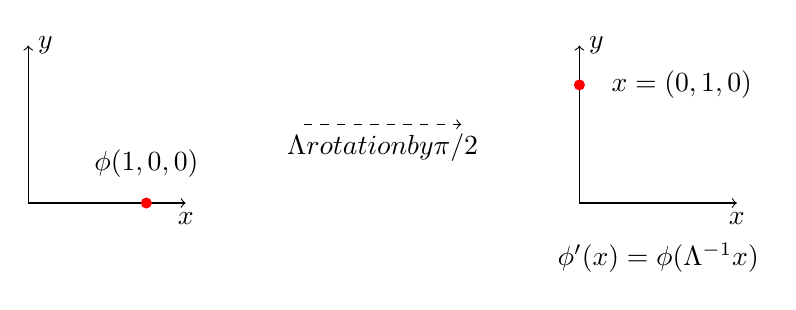
\begin{tikzpicture}
    % R^n axes
    \draw[->] (-4.5,0) -- (-2.5,0) node[anchor=north] {$x$};
    \draw[->] (-4.5,0) -- (-4.5,2) node[anchor=west] {$y$};
    \fill[red] (-3,0) circle (2pt);
    \node at (-3, 0.5) {$\phi(1, 0, 0)$};

    % R^{n'} axes
    \draw[->] (2.5,0) -- (4.5,0) node[anchor=north] {$x$};
    \draw[->] (2.5,0) -- (2.5,2) node[anchor=west] {$y$};
    \fill[red] (2.5,1.5) circle (2pt);
    \node at (3.5, -0.7) {$\phi'(x) = \phi(\Lambda^{-1}x)$};
    \node at (3.8, 1.5) {$x = (0, 1, 0)$};

    % Dashed arrow for the map between R^n and R^{n'}
    \draw[->, dashed] (-1,1) -- (1,1) node[midway,below] {$\Lambda \text{ rotation by } \pi/2$};


\end{tikzpicture}
\end{center}

\begin{exbox}
	The trivial representation gives a scalar field.

	Another example is a vector representation, so
	\[
		D[\Lambda] \indices{^{\mu}_{\nu}} = \Lambda\indices{^{\mu}_{\nu}}.
	\]
	So then
	\[
	A^\mu(x) \to A'^\mu(x) = \Lambda\indices{^{\mu}_{\nu}} A^\nu(\Lambda^{-1}x),
	\]
	and
	\[
	\partial_\mu \phi \to \partial_\mu \phi'(x) = (\Lambda^{-1})\indices{^{\mu}_{\nu}} \partial_\mu \phi(\Lambda^{-1}x).
	\]
\end{exbox}

Now we will see how symmetries constrain actions. For example consider
\[
\mathcal{L} = \frac{1}{2} \partial_\mu \phi \partial_\nu \phi \eta^{\mu\nu} - \frac{1}{2} m^2 \phi^2, \qquad S = \int \Diff 4 x \, \mathcal{L}.
\]
We can verify this is invariant under Lorentz.

% lecture 3

Note under the Lorentz transformation, the fields transform as
\begin{align*}
	\phi(x) &\to \phi(x) = \phi(\Lambda^{-1}x) = \phi(y), \\
	\partial_\mu \phi &\to (\Lambda^{-1})\indices{^{\nu}_{\mu}} \partial_\nu \phi(y).
\end{align*}
If we replace this in the Lagrangian,
\begin{align*}
	\mathcal{L} &\to \frac{1}{2}(\Lambda^{-1})\indices{^{\rho}_{\mu}} \partial_\mu \phi(y) (\Lambda^{-1})\indices{^{\sigma}_{\nu}} \partial_\sigma \phi(y) - \frac{1}{2} m^2 \phi^2(y) \\
		    &= \frac{1}{2} \eta^{\rho\sigma} \partial_\rho \phi \partial_\sigma \phi - \frac{1}{2} m^2 \phi^2.
\end{align*}
Therefore,
\[
\mathcal{L}(x) \to \mathcal{L}'(x) = \mathcal{L}(y).
\]
Hence
\[
S = \int \Diff4 x \, \mathcal{L}(x) \to \int \Diff4 x \, \mathcal{L}(y) = \int \Diff4 y\, \mathcal{L}(y)
\]
is conserved (note the change in variable $x \to y$ has Jacobian 1, as $\det \Lambda = 1$).

\subsection{N\"oether's Theorem}%
\label{sub:nt}

This has two parts:
\begin{enumerate}
	\item Every continuous symmetry of the Lagrangian gives rise to a current $j^\mu$, and the equations of motions imply
		\[
		\partial_\mu j^\mu = 0 \implies \frac{\partial j^0}{\partial t} + \nabla \cdot j^i = 0.
		\]
	\item Provided suitable boundary conditions,  a conserved current will give rise to a conserved charge $Q$, where
		\[
		Q = \int \Diff 3x \,j^0.
		\]
\end{enumerate}

\begin{definition}
	A transformation is \emph{continuous} if there is an infinitesimal parameter in it. They can either be:
	\begin{itemize}
		\item internal: they do not act on the coordinates, but instead on the fields.
		\item local: they act on the coordinates and the fields.
	\end{itemize}
	In both cases, the differential of a continuous transformation is
	\[
	\delta \phi_a = \phi_a'(x) - \phi_a(x).
	\]
	Such a transformation is a symmetry of the system if the action is invariant, so
	\[
	S[\phi] \to S[\phi'] = \int \Diff4 x\, \mathcal{L}(x),
	\]
	and moreover
	\[
		\delta(S) = S[\phi'] - S[\phi] = 0.
	\]
	This implies that for the Lagrangian,
	\[
	\delta \mathcal{L} = \mathcal{L}'(x) - \mathcal{L}(x) = \partial_\mu F^\mu,
	\]
	the same up to a total derivative.
\end{definition}

\begin{proofbox}
	Let us quantify the change in $\mathcal{L}$:
	\begin{align*}
		\delta \mathcal{L} &= \frac{\partial \mathcal{L}}{\partial \phi_a}  \delta \phi_a + \frac{\partial \mathcal{L}}{\partial \partial_\mu \phi_a} \delta \partial_\mu \phi_\alpha \\
				   &= \left( \frac{\partial \mathcal{L}}{\partial \phi_a} - \partial_\mu \left( \frac{\partial \mathcal{L}}{\partial \partial_\mu \phi_a} \right) \right) \delta \phi_a + \partial_\mu \left( \frac{\partial \mathcal{L}}{\partial \partial_\mu \phi_a} \delta \phi_\alpha \right) = \partial_\mu F^\mu,
	\end{align*}
	as it is a symmetry. Hence,
	\[
		- \left( \frac{\partial \mathcal{L}}{\partial \phi_a} - \partial_\mu \left( \frac{\partial \mathcal{L}}{\partial \partial_\mu \phi_a} \right) \right) \delta \phi_a = \partial_\mu \underbrace{\left( \frac{\partial \mathcal{L}}{\partial \partial_\mu \phi_a} \delta \phi_a - F^\mu \right)}_{j^\mu}.
	\]
	If the equations of motion are imposed, then
	\[
	\partial_\mu j^\mu = 0,
	\]
	where
	\[
	j^\mu = \frac{\partial \mathcal{L}}{\partial \partial_\mu \phi_\alpha} \delta \phi_a - F^\mu.
	\]
	For the second part of the statement, we have
	\[
	Q = \int \Diff 3 x \, j^0.
	\]
	Then the total time derivative is
	\[
	\frac{\diff Q}{\diff t} = \int_V \Diff3 x\, \frac{\partial j^0}{\partial t} = - \int_V \Diff3 x \, \nabla \cdot j = - \int_{\partial V} \diff A \cdot j = 0,
	\]
	given suitable boundary conditions on $j$, i.e. fields decay.
\end{proofbox}

\subsection{Energy-Momentum Tensor}%
\label{sub:em_t}

Consider local transformations given by translations:
\[
x^\mu \to x'^\mu = x^\mu - \eps^\mu.
\]
Under translation, the fields transform as
\[
\phi_a(x) \to \phi_a'(x) = \phi_a(x + \eps) = \phi_a(x) + \eps^\mu \partial_\mu \phi_a + \mathcal{O}(\eps^2).
\]
Hence we find
\[
\delta \phi_a = \phi_a'(x) - \phi_a(x) = \eps^\mu \partial_\mu \phi_a.
\]
The Lagrangian changes as
\[
\delta \mathcal{L} = \eps^\mu \partial_\mu \mathcal{L} = \partial_\mu (\eps^\mu \mathcal{L}).
\]
The conserved current is then
\begin{align*}
	j^\mu &= \frac{\partial \mathcal{L}}{\partial(\partial_\mu \phi_a)} \eps^\nu \partial_\nu \phi_a - \eps^\mu \mathcal{L} \\
	      &= \eps^\nu \left( \frac{\partial \mathcal{L}}{\partial (\partial_\mu \phi_a)} \partial_\nu \phi_a - \delta\indices{^{\mu}_{\nu}} \mathcal{L} \right) \\
	      &= \eps^\nu T\indices{^{\mu}_{\nu}},
\end{align*}
where $T\indices{^{\mu}_{\nu}}$ is the energy-momentum tensor. If the equations of motion are 0, then varying $\eps^\nu$, we find
\[
\partial_\mu j^\mu = 0 \implies \partial_\mu T\indices{^{\mu}_{\nu}} = 0.
\]
We can construct four conserved charges:
\begin{align*}
	E &= \int \Diff3 x \, T^{00}, \\
	P^i &= \int \Diff 3 x \, T^{0i}.
\end{align*}
These are the energy, and the three momenta.

\begin{exbox}[Free massive scalar field]
	Here we have
	\[
	T\indices{^{\mu}_{\nu}} = \frac{\partial \mathcal{L}}{\partial (\partial_\mu \phi_a)} \partial_\nu \phi - \delta\indices{^{\mu}_{\nu}} \mathcal{L},
	\]
	so
	\[
	T^{\mu\nu}= \partial^\mu \phi \partial^\nu \phi - \eta^{\mu\nu} \mathcal{L}.
	\]
	Then we find
	\[
	T^{00} = \frac{1}{2} \dot \phi^2 + \frac{1}{2} (\nabla \phi)^2 + \frac{1}{2} m^2 \phi^2.
	\]
	So
	\[
	E = \int \Diff 3 x \, T^{00} = H, \qquad P^i = \int \Diff 3 x \, T^{0i} = \int \Diff 3x \, \dot \phi \partial^i \phi.
	\]
\end{exbox}

\begin{remark}
	The definition of the EM tensor is
	\[
	T\indices{^{\mu}_{\nu}} = \frac{\partial \mathcal{L}}{\partial (\partial_\mu \phi_a)} \partial_\nu \phi_a - \delta\indices{^{\mu}_{\nu}} \mathcal{L}.
	\]
	From this equation, we do not ensure that $T$ is symmetric. How can we make it symmetric?
	\begin{enumerate}
		\item Define
			\[
			\Theta^{\mu\nu} = T^{\mu\nu} + \partial_\rho \Gamma^{\rho\mu\nu},
			\]
			where
			\[
			\Gamma^{\rho\mu\nu}= - \Gamma^{\mu\rho\nu},
			\]
			such that $\partial_\mu \Theta^{\mu\nu} = 0$.
		\item Couple fields to $g_{\mu\nu}$. Then
			\[
			\Theta^{\mu\nu} = \left( - \frac{2}{\sqrt{-g}} \frac{\partial}{\partial g_{\mu\nu}} \left( \sqrt{-g} \mathcal{L} \right) \right) \biggr|_{g = \eta}.
			\]
	\end{enumerate}
	
\end{remark}

% lecture 4

\begin{exbox}[Complex scalar field]
	A complex scalar field is
	\[
	\psi(x) = \frac{1}{\sqrt 2} (\phi_1(x) + i \phi_2(x)),
	\]
	where $\phi_i$ are real scalar fields. A Lagrangian for this field is
	\[
	\mathcal{L} = \frac{1}{2} \partial_\mu \psi \partial^\mu \psi^\ast - V(|\psi|^2).
	\]
	The equations of motion turn out to be
	\[
	\partial_\mu \partial^\mu \psi + \frac{\partial V}{\partial \psi^\ast} = 0, \qquad \partial_\mu \partial^\mu \psi^\ast + \frac{\partial V}{\partial \psi} = 0.
	\]
	In this system, there is an internal symmetry given by
	\[
	\psi(x) \to \psi'(x) = e^{i \alpha} \psi(x), \qquad \psi^\ast (x) \to \psi'^\ast (x) = e^{-i\alpha} \psi^\ast(x).
	\]
	Here $\mathcal{L} \to \mathcal{L}' = \mathcal{L}$, so $\mathcal{S} \to \mathcal{S}' = \mathcal{S}$.

	$\alpha$ is a continuous parameter of the transformation, so $\delta \psi = \psi'(\alpha) - \psi(\alpha) = i \alpha \psi$, and $\delta \psi^\ast = -i\alpha \psi^\ast$.

	We can construct the current as
	\begin{align*}
		j^\mu &= \frac{\partial \mathcal{L}}{\partial \partial_\mu \psi} \delta \psi + \frac{\partial \mathcal{L}}{\partial \partial_\mu \psi^\ast} \delta \psi^\ast \\
		      &= \partial^\mu \psi^\ast \delta \psi + \partial^\mu \psi \delta \psi^\ast \\
		      &= i \alpha(\psi \partial^\mu \psi^\ast - \psi^\ast \partial^\mu \psi).
	\end{align*}
	It is also possible to parametrize our transformation as
	\[
	\begin{pmatrix}
		\phi_1 \\ \phi_2
	\end{pmatrix}
	\to
	\begin{pmatrix}
		\phi_1' \\ \phi_2'
	\end{pmatrix} =
	\begin{pmatrix}
		\cos \alpha & -\sin\alpha \\ \sin \alpha & \cos \alpha
	\end{pmatrix}
	\begin{pmatrix}
		\phi_1 \\ \phi_2
	\end{pmatrix}.
	\]
\end{exbox}

\newpage

\section{Quantum Fields}%
\label{sec:qf}

\subsection{Free Theory}%
\label{sub:qfft}

We will begin by taking a Hamiltonian approach, and will follow the rules of QM. In this framework,
\[
	[X^i, P^j] = i \hbar \delta^{ij}.
\]
In QFT, we now have $\phi_a(x)$ and $\Pi^a(x)$, where $\Pi^a = \partial \mathcal{L} / \partial \phi_a$. The new rule is
\[
	[\phi_a(\mathbf{x}, t), \Pi^b(\mathbf{x}, t)] = i \delta^3(\mathbf{x} - \mathbf{y}) \delta\indices{^{b}_{a}}.
\]
This looks like it breaks relativity; we will see it does not. Our goal is to implement such a quantum field theory for the free massive real scalar field. The plan will be to go through:
\begin{itemize}
	\item Canonical quantization.
	\item Hamiltonian.
	\item Fock space.
	\item Causality.
	\item Propagators.
\end{itemize}

\subsection{Canonical Quantization}%
\label{sub:cq}

Our theory is
\[
\mathcal{L} = \frac{1}{2} \partial_\mu \phi \partial^\mu \phi - \frac{1}{2} m^2 \phi^2.
\]
The equations of motion are
\[
\partial_\mu \partial^\mu \phi + m^2 \phi = 0.
\]
Solutions to this include
\[
\phi \sim \exp\left( i \mathbf{k} \cdot \mathbf{x} + i \omega t\right),
\]
where $\omega, \mathbf{k}, m$ are related by
\[
	-\omega^2 + \mathbf{k}^2 + m^2 = 0 \implies \omega = \pm \sqrt{\mathbf{k}^2 + m^2}.
\]
We adopt the notation
\[
	\omega = \sqrt{\mathbf{k}^2 + m^2}.
\]
Hence, we can write
\[
	\phi(\mathbf{x}, t) = \int \frac{\Diff3 k}{(2 \pi)^3} \left[ a(\mathbf{k}) e^{i \mathbf{k} \cdot \mathbf{x} - i \omega t} + b(\mathbf{k}) e^{i \mathbf{k} \cdot \mathbf{x} + i \omega t} \right].
\]
Note that $\phi$ is real, so $\phi^\ast = \phi$ implies
\[
a^\ast(- \mathbf{k}) = b(\mathbf{k}), \qquad b^\ast(-\mathbf{k}) = a(\mathbf{k}).
\]
Hence we can write
\begin{align*}
	\phi(x) &= \int \frac{\Diff3 k}{(2 \pi)^3} \left[ a(\mathbf{k}) e^{i \mathbf{k} \cdot \mathbf{x} - i \omega t} + a^\ast(\mathbf{k}) e^{-i \mathbf{k} \cdot \mathbf{x} + i \omega t} \right] \\
		&= \int \frac{\Diff3 k}{( 2\pi)^3} \left[ a(\mathbf{k}) e^{-ikx} + a^\ast(\mathbf{k}) e^{ik x} \right],
\end{align*}
where
\[
kx = k^\mu x_\mu = \omega t - \mathbf{k} \cdot \mathbf{x}, \qquad k^2 = \omega^2 - \mathbf{k}^2 = m^2.
\]
We choose to normalize $a(\mathbf{k})$ and $a^\ast(\mathbf{k})$ such that
\[
	\phi(x) = \int \frac{\Diff 3k}{(2\pi)^3} \frac{1}{\sqrt{2 \omega}} \left[ a(\mathbf{k}) e^{-ikx} + a^\ast(\mathbf{k}) e^{ikx}\right].
\]
Next, we quantize. To do this, we calculate the conjugate momenta:
\[
	\Pi(x) = \dot \phi = \int \frac{\Diff3k}{(2\pi)^3} \frac{1}{i}\sqrt{\frac \omega2} \left[ a(\mathbf{k}) e^{-ikx} - a^\ast(\mathbf{k})e^{ikx}\right].
\]
We declare
\begin{align*}
	[\phi(\mathbf{x}, t), \phi(\mathbf{x}', t)] &= 0,\\
	[\Pi(\mathbf{x},t), \Pi(\mathbf{x}',t)] &= 0,\\
	[\phi(\mathbf{x}, t), \Pi(\mathbf{x}', t)] &= i \delta^3(\mathbf{x} - \mathbf{x}').
\end{align*}
The claim is that these commutation relations promote $a$ to an operator, and $a^\ast$ becomes $a^\dagger$, also an operator. These themselves have commutation relations:
\begin{align*}
	[a(\mathbf{k}), a(\mathbf{k}')] &= 0,\\
	[a^\dagger(\mathbf{k}), a^\dagger(\mathbf{k}')] &= 0,\\
	[a(\mathbf{k}), a^\dagger(\mathbf{k}')] &= (2 \pi)^3 \delta^3(\mathbf{k} - \mathbf{k}').
\end{align*}

\begin{proofbox}
	We show that the second set of commutation relations imply the first set. We only prove the last one as it is the only non-trivial one:
	\begin{align*}
		[\phi(\mathbf{x}, t), \Pi(\mathbf{y}, t)] &= \int \frac{\Diff3 p \Diff 3 q}{(2 \pi)^6} \frac{1}{2i} \sqrt{\frac{\omega_p}{\omega_q}} \bigl( \bigl[ a(p) e^{i \mathbf{p} \cdot \mathbf{x} - i \omega t} + a^\dagger (p) e^{-i \mathbf{p} \cdot \mathbf{x} + i \omega t}, \\
							  &\qquad \qquad \qquad a(q) e^{i \mathbf{q} \cdot \mathbf{y} - i \omega t} - a^\dagger(q) e^{-i \mathbf{q} \cdot \mathbf{y} + i \omega t} \bigr] \bigr) \\
							  &= C \int \Diff3 p \Diff3 q \bigl( - [a(p), a^\dagger(q)] e^{i \mathbf{p} \cdot \mathbf{x}} e^{-i \mathbf{q} \cdot \mathbf{y}} e^{it(\omega_q - \omega_p)} \\
							  & \qquad \qquad \qquad \qquad + [a^\dagger(p), a(q)] e^{-i \mathbf{p} \cdot \mathbf{x}} e^{i \mathbf{q} \cdot \mathbf{y}} e^{it(\omega_p - \omega_q)} \bigr) \\
							  &= i \int \frac{\Diff 3 p}{(2 \pi)^3} e^{i p (\mathbf{x} - \mathbf{y})} = i \delta^3(\mathbf{x} - \mathbf{y}).
	\end{align*}
\end{proofbox}

% lecture 5

\subsection{Hamiltonian}%
\label{sub:hqft}

The Hamiltonian of the free theory is
\[
	H = \int \Diff3 x \, \mathcal{H} = \frac{1}{2} \int \Diff 3 x\,(\Pi^2 + (\nabla \phi)^2 + m^2 \phi^2),
\]
which we want in terms of $a, a^\dagger$. Writing this out,
\begin{align*}
	H &= \frac{1}{2} \int \Diff 3 x \int \frac{\Diff 3 p \Diff 3 q}{(2\pi)^6} \biggl( - \frac{\sqrt{\omega_p \omega_q}}{2} (a e^{-ipx} - a^{\dagger} e^{ipx})(ae^{-iqx} - a^{\dagger} e^{iqx}) \\
	  & \qquad \qquad - \frac{1}{2} \frac{1}{\sqrt{\omega_p \omega_q}} (a e^{-ipx} - a^{\dagger} e^{ipx})(a e^{-iqx} - a^\dagger e^{iqx}) \mathbf{p} \cdot \mathbf{q} \\
	  & \qquad \qquad + \frac{m^2}{2} \frac{1}{\sqrt{\omega_p \omega_q}} (a e^{ipx} + a^{\dagger} e^{-ipx})(ae^{iqx} + a^{\dagger} e^{-iqx}) \biggr) \\
	  &= \frac{1}{2} \int \frac{\Diff 3 p}{(2 \pi)^3} \frac{1}{2 \omega_p} \biggl[ \underbrace{(-\omega_p^2 + \mathbf{p}^2 + m^2)}_{0}(a_p a_p e^{-2i\omega t} + a_p^{\dagger} a_p^{\dagger} e^{2i\omega t}) \\
	  & \qquad \qquad + (\omega_p^2 + \mathbf{p}^2 + m^2)(a_p^\dagger a_p + a_p a_p^\dagger) \biggr] \\
	  &= \frac{1}{2} \int \frac{\Diff 3p}{(2 \pi)^3} \omega_p(a_p^\dagger a_p + a_p a_p^\dagger) \\
	  &= \int \frac{\Diff 3 p}{(2 \pi)^3} \omega_p a_p^\dagger a_p + \int \frac{\Diff 3 p}{2} \, \omega_p \delta(0).
\end{align*}
We should be scared by the last term. If we take a vacuum state $\ket 0$ such that
\[
a_p \ket 0 = 0,
\]
then in fact
\[
H \ket 0 = \int \frac{\Diff 3 p}{2} \, \omega (2 \pi)^3 \delta(0) \ket 0 = \infty.
\]
To understand the nature of this, we need to see the origin of this divergence. We actually have two infinities:
\begin{enumerate}[(i)]
	\item Infrared divergence: $(2 \pi)^3 \delta(0)$. This arises as follows:
		\[
			(2\pi)^3 \delta(0) = \lim_{L \to \infty} \int_{-L}^L \Diff 3 x \, e^{i \mathbf{x} \cdot \mathbf{p}} \biggr|_{\mathbf{p} = 0} = \lim_{L \to \infty} \int_{-L}^{L} \Diff 3 x = V.
		\]
		For an infinite size system, this blows up. The solution is to discuss energy densities, so
		\[
		\mathcal{E}_0 = \frac{E_0}{V} = \int \frac{\Diff 3p}{(2 \pi)^3} \, \frac{1}{2} \omega_p \sim \int \Diff 3 p \, p^{2} \to \infty.
		\]
		This also diverges.
	\item Ultraviolet divergence:
		\[
			\int_0^{p_{\mathrm{max}}} \Diff 3 p \, \sqrt{p^2 + m^2} \to \infty,
		\]
		which is high-frequency divergence.

		It is absurd to think that the theory is valid for arbitrarily high energies.
\end{enumerate}

The solution, which is mostly practical, is to declare
\[
H = \int \frac{\Diff 3 p}{(2 \pi)^3} \, \omega_p a_p^\dagger a_p,
\]
and with this $H \ket 0 = 0$.

The origin is due to an ambiguity in multiplying fields. The cure is \emph{normal ordering}\index{normal ordering}.

\begin{definition}
	If we are given a list of fields, we define the \emph{normal ordering} as
	\[
		\normalorder{\phi_1(x_1) \phi_2(x_2) \cdots \phi_n(x_n)}
	\]
	where this is the usual product with all $a(p)$ operators placed to the right of an $a^\dagger(p)$.
\end{definition}

\subsection{Fock Space}%
\label{sub:fs}

Given $\ket 0$, we want to construct excited states. We know
\begin{align*}
	[H, a_p^\dagger] &= \omega_p a_p^\dagger, \\
	[H, a_p] &= \omega_p a_p.
\end{align*}
We can construct excited states by
\begin{align*}
	\ket p &= a^\dagger(p) \ket 0, \\
	H \ket p &= \omega_p \ket p,
\end{align*}
% lecture 6
where $\omega_p^2 = p^2 + m^2$. We can consider
\[
\mathbf{P} = - \int \Diff3 x \, \pi \nabla \phi = \int \frac{\Diff 3 k}{(2 \pi)^3} k a_k^\dagger a_k,
\]
where
\[
	\mathbf{P}\ket{\mathbf{p}}= \mathbf{p} \ket{\mathbf{p}}.
\]
Here $\ket{\mathbf{p}}$ is a momentum and energy eigenstate, with eigenvalues $\mathbf{p}$ and energy $E = w_p^2 = \mathbf{p}^2 + m^2$.

Also, $\mathbf{p} = 0$ is an angular momentum $J^i$ eigenstate, i.e.
\[
	J^i \ket{\mathbf{p} = 0} = 0.
\]
With this, we can create more states:
\[
	\ket{\mathbf{p}_1 \cdots \mathbf{p}_n} = a^{\dagger}(\mathbf{p}_1) \cdots a^{\dagger}(\mathbf{p}_n) \ket 0.
\]
Because $a^\dagger$ commute, these are configurations which are symmetric under interchange, i.e.
\[
	\ket{\mathbf{p}_1 \mathbf{p}_2} = \ket{\mathbf{p}_2 \mathbf{p}_1}.
\]
The \emph{Fock space}\index{Fock space} is the collection of all possible combinations of $a^\dagger$ acting on $\ket 0$. Introducing
\[
N = \int\frac{\Diff 3p}{(2\pi)^3} a_p^\dagger a_p,
\]
which is the \emph{number operator}\index{number operator}, we find
\[
	N \ket{\mathbf{p}_1 \cdots \mathbf{p}_n} = n \ket{\mathbf{p}_1 \cdots \mathbf{p}_n}.
\]
For a free theory,
\[
	[N, H] = 0.
\]
Fork space is then
\[
\oplus_i \mathcal{H}_n
\]

\subsection{Relativistic Normalization}%
\label{sub:rn}

How do we normalize these states? First thing, pick
\[
	\braket{0|0} = 1.
\]
For 1-particle states, note
\[
	\ket{\mathbf{p}} = a_p^\dagger \ket 0 \implies \braket{\mathbf{p}|\mathbf{q}} = (2\pi)^3 \delta^3(\mathbf{p} - \mathbf{q}).
\]
This is not Lorentz invariant. Our dream is that under a Lorentz transformation,
\[
	\ket{\mathbf{p}} \to \ket{\mathbf{p}'} = U(\Lambda) \ket{\mathbf{p}}.
\]
To figure out a proper definition of $\ket{\mathbf{p}}$, we use the identity
\[
	\ket{\mathbf{q}}=  \int \frac{\Diff3p}{(2\pi)^3} \ket{\mathbf{p}} \braket{\mathbf{p}|\mathbf{q}},
\]
hence
\[
	1 = \int \frac{\Diff3p}{(2\pi)^3} \ket{\mathbf{p}}\bra{\mathbf{p}}.
\]
This integral is manifestly not Lorentz invariant, due to the measure we are taking the integral over. Instead, we transform
\begin{align*}
	\int \frac{\Diff3p}{(2\pi)^3} &\to \int \Diff4p \, \delta^{4}(\mathbf{p}^2-m^2) \Theta(p^0) = \int \Diff3p\, \frac{1}{2\sqrt{\mathbf{p}^2 + m^2}} \\
				      &= \int \Diff3 p \frac{1}{2 \omega_p}.
\end{align*}
So instead, we should define
\[
	1 = \int \frac{\Diff3p}{(2\pi)^3} \frac{1}{2\omega_p} \ket{\mathbf{p}}\bra{\mathbf{p}},
\]
where
\[
	\ket{\mathbf{p}} = \sqrt{2\omega_p} a_p^\dagger \ket 0.
\]
This is relativistic normalization.

\subsection{Causality}%
\label{sub:cause}

Here we are interested in whether measurements influence each other, i.e. whether commutators vanish. This is associated with why equal-time commutators are compatible with relativity. Define
\[
	\Delta(x - y) = [\phi(x), \phi(y)].
\]
We can evaluate this for a free theory:
\begin{align*}
	\Delta &= [\phi(x), \phi(y)] \\
	       &= \int \frac{\Diff3k}{(2\pi)^3} \frac{\Diff3p}{(2\pi)^3}\frac{1}{2\sqrt{\omega_k\omega_p}}([a_k, a_p^\dagger] e^{-ikx} e^{ipy} + [a_k^\dagger, a_p] e^{ikx} e^{-ipy} ) \\
	       &= \int \frac{\Diff 3 p}{(2 \pi)^3} \frac{1}{2\omega_p} (e^{-ip\cdot(x - y)} - e^{ip\cdot(x-y)}).
\end{align*}
This commutator satisfies a few properties:
\begin{itemize}
	\item It is Lorentz invariant due to the appearance of our measure, and also a c-number operator.
	\item For time-like separation, $(x-y)_T = (t, 0, 0, 0)$, we find
		\[
		\Delta(x - y)_T = \int \frac{\Diff3p}{(2\pi)^3} \frac{1}{2\omega_p}(e^{-i\omega_pt}-e^{i\omega_pt}) \sim e^{-imt}-e^{imt}\neq 0.
		\]
	\item For spacelike separation, say $(x-y)_S = (0, \mathbf{x} - \mathbf{y})$, then
		\[
		\Delta(x - y)_S = \int\frac{\Diff3p}{(2\pi)^3}\frac{1}{2\omega_p}(e^{i\mathbf{p}\cdot(\mathbf{x}-\mathbf{y})}-e^{-i\mathbf{p}\cdot(\mathbf{x}-\mathbf{y})})=0,
		\]
		so any two spacelike events have zero commutator.
\end{itemize}

\subsection{Propagators}%
\label{sub:props}

Here we are interested in the quantity
\[
	\braket{0|\phi(x)\phi(y)|0} = \int \frac{\Diff3p}{(2\pi)^3} \frac{1}{2\omega_p} e^{-ip(x-y)} = D(x-y).
\]
This can be thought of as preparing a particle at position $y$, and measuring its amplitude at position $x$. For spacelike events,
\[
D(x-y) \sim e^{-m(\mathbf{x}-\mathbf{y})} \neq 0.
\]
But,
\[
	[\phi(x),\phi(y)]=D(x-y)-D(y-x)=0.
\]

% lecture 7

Define
\[
	\Delta_F(x - y) = \braket{0|T \phi(x) \phi(y)|0}=
	\begin{cases}
		D(x - y) & x^0 > y^0, \\
		D(y - x) & y^0 > x^0.
	\end{cases}
\]
Here $T$ is the \emph{time operator}\index{time operator}. We claim that
\[
\Delta_F(x - y) = \int \frac{\Diff 4 p}{(2 \pi)^4} \frac{i}{p^2 - m^2 + i \eps} e^{-ip(x - y)}.
\]

\begin{proofbox}
	A lot of calculation:
	\begin{align*}
		\braket{0|T\phi(x) \phi(y)|0} &= \braket{0|\phi(x) \phi(y)|0} \Theta(x^0 - y^0) + \braket{0|\phi(y)\phi(x)|0} \Theta(y^0 - x^0) \\
					      &= \int \frac{\Diff 3 k}{(2 \pi)^3} \frac{1}{2 \omega_k} e^{-i \omega_k (x^0 - y^0)} e^{i \mathbf{k} \cdot (\mathbf{x} - \mathbf{y})} \Theta(x^0 - y^0) \\
					      & \qquad \qquad + \int \frac{\Diff 3 k}{(2 \pi)^3} \frac{1}{2 \omega_k} e^{-i \omega_k (y^0 - x^0)} e^{i \mathbf{k}(\mathbf{y} - \mathbf{x})} \Theta(y^0 - x^0) \\
					      &= \int \frac{\Diff 3 k}{(2 \pi)^3} \frac{1}{2 \omega_k} e^{i \mathbf{k} \cdot (\mathbf{x} - \mathbf{y})} \left( e^{-i \omega_k z} \Theta(z) + e^{i\omega_k z} \Theta(-z) \right).
	\end{align*}
	We focus on the time-dependent part, and show that
	\[
		e^{-i\omega_k z}\Theta(z) + e^{i\omega_k z} \Theta(-z) = \lim_{\eps \to 0} \frac{(- 2 \omega_k)}{2 \pi i} \int_{-\infty}^{\infty} \diff \omega \frac{e^{ i \omega z}}{\omega^2 - \omega_k^2 + \eps}.
	\]
	We start from the right hand side of the equation:
	\begin{align*}
		\frac{1}{\omega^2 - \omega_k^2 + i \eps} &= \frac{1}{(\omega - (\omega_k - i \tilde \eps))(\omega - (-\omega_k + i \tilde \eps))} \\
							 &= \frac{1}{2 \omega_k} \left[ \frac{1}{\omega - (\omega_k - i \eps)} - \frac{1}{\omega - (-\omega_k + i \eps)} \right] + \mathcal{O}(\eps^2).
	\end{align*}
	Consider the integral
	\[
	I_1 = \int_{-\infty}^{\infty} \frac{e^{-i \omega z}}{\omega - (\omega_k - i \eps)}.
	\]
	We want to use Schwartz' lemma to evaluate this in the complex plane. The function has a pole at $\omega = \omega_k - i \eps$.

	If $z < 0$, we can complete is in the upper-half plane, and get $I_1 = 0$. If $z > 0$, we need to close it in the lower-half plane, which encompasses the pole, and results in an integral of
	\[
	I_1 = - 2 \pi i e^{-i \omega_k z} \theta(z) + \mathcal{O}(\eps).
	\]
	The negative sign is as we are integrated in a clockwise direction.

	The other term in the integral is
	\[
	I_2 = \int_{-\infty}^{\infty} \diff \omega \frac{e^{-i \omega z}}{\omega - (-\omega_k + i \eps)}.
	\]
	We can do a similar thing to find $I_2$, and get
	\[
	I_2 = 2 \pi i e^{i \omega_k z} \Theta(-z) + \mathcal{O}(\eps).
	\]
	Collecting these terms,
	\begin{align*}
		\lim_{\eps \to 0} \int_{-\infty}^{\infty} \diff \omega \frac{e^{-i\omega z}}{\omega^2 - \omega_k^2 + \eps} &= \lim_{\eps \to 0} \frac{1}{2 \omega_k} (I_1 - I_2) \\
															   &= \frac{1}{2 \omega_k} \left(- 2 \pi i e^{-i \omega_k z} \Theta(z) - 2 \pi i e^{i \omega_k z} \Theta(-z) \right).
	\end{align*}
	Pulling this into the expression,
	\begin{align*}
		\braket{0|T\phi(x)\phi(y)|0} &= \int \frac{\Diff 3 k}{(2 \pi)^3} \frac{i}{2 \pi} e^{i \mathbf{k} \cdot (\mathbf{x} - \mathbf{y})} \int_{-\infty}^{\infty} \diff \omega \frac{e^{-i \omega z}}{\omega^2 - \omega_k^2 + i \eps} \\
					     &= \int \frac{\Diff 4 k}{(2 \pi)^{4}} \frac{i}{k^2 - m^2 + i \eps} e^{-i k(x - y)}.
	\end{align*}
\end{proofbox}

By convention we drop the limit.

\begin{remark}
	\begin{enumerate}
		\item[]
		\item Due to the time ordering, our contour is prescribed.
		\item $\Delta_F(x - y)$ is Lorentz invariant.
		\item $\Delta_F(x - y)$ is a Green's function, as
			\begin{align*}
				(\partial_\mu \partial^\mu + m^2)\Delta_F(x - y) &= -i \delta^{4}(x - y).
			\end{align*}
			$\Delta_F$ is the Green's function associated to the Klein-Gordon equation.
% lecture 8
		\item Normal orderings are invariant up to reordering, as each $a^{\dagger}$ and $a$ commute.
		\item Fun little fact:
			\[
				T \phi(x) \phi(y) = \normalorder{\phi(x) \phi(y)} + \Delta_F(x - y) = \normalorder{\phi(x) \phi(y)} + \overbrace{\phi(x)\phi(y)}
			\]
			To prove this, write $\phi = \phi^{+} + \phi^{-}$, where 
			\begin{align*}
				\phi^{+} &= \int \frac{\Diff 3 p}{(2\pi)^3} \frac{1}{\sqrt{2 \omega_p}} a_p e^{-i p x}, \\
				\phi^{-} &= \int \frac{\Diff 3 p}{(2\pi)^3} \frac{1}{\sqrt{2 \omega_p}} a_p^{\dagger} e^{i p x}.
			\end{align*}
			Choose $x^0 > y^0$. Then,
			\begin{align*}
				T(\phi(x)\phi(y)) &= \phi(x)\phi(y) \\
						  &= \phi^{+}(x) \phi^{+}(y) + \phi^{-}(x) \phi^{+}(y) + \phi^{-}(y) \phi^{+}(x) \\
						  & \qquad + [\phi^{+}(x), \phi^{-}(y)] + \phi^{-}(x) \phi^{-}(y) \\
						  &= \normalorder{\phi(x) \phi(y)} + D(x - y).
			\end{align*}
			If $x^0 < y^0$, we get
			\[
			T \phi(x) \phi(y) = \normalorder{\phi(x)\phi(y)} + D(y - x).
			\]
			Together this gives \emph{Wick's theorem}, a generalisation of this:
			\begin{align*}
				T(\phi(x_1) \phi(x_2) \phi(x_3)\phi(x_4)) &= \normalorder{\phi(x_1)\phi(x_2)\phi(x_3)\phi(x_4)} \\
									  & \qquad + \overbrace{\phi_1 \phi_2} \normalorder{\phi_3 \phi_4} + \overbrace{\phi_1 \phi_3} \normalorder{\phi_2 \phi_4} + \overbrace{\phi_1 \phi_4} \normalorder{\phi_2\phi_3} \\
									  & \qquad + \overbrace{\phi_2\phi_3} \normalorder{\phi_1 \phi_4} + \overbrace{\phi_2 \phi_4} \normalorder{\phi_1\phi_3} + \overbrace{\phi_3\phi_4} \normalorder{\phi_1\phi_2} \\
									  & \qquad + \overbrace{\phi_1\phi_2} \overbrace{\phi_3 \phi_4} + \overbrace{\phi_1\phi_3} \overbrace{\phi_2\phi_4} + \overbrace{\phi_1\phi_4} \overbrace{\phi_2\phi_3}.
			\end{align*}
	\end{enumerate}
\end{remark}

\newpage

\section{Interactions}%
\label{sec:ints}

\subsection{Couplings}%
\label{sub:cups}

The free theory we have been studying so far is ``simple'': we can construct explicitly the Fock space.

We want to consider more general Lagrangians. An obstruction is that we cannot generally solve the equations of motion, hence do not have access to the Hilbert space.

In this way, we take a perturbative approach to QFT, where
\[
\mathcal{L} = \mathcal{L}_0 + \mathcal{L}_{\mathrm{int}},
\]
where say
\[
\mathcal{L}_0 = \frac{1}{2} \partial_\mu \phi \partial^\mu \phi - \frac{1}{2} m^2 \phi^2,
\]
and
\[
\mathcal{L}_{\mathrm{int}} = \sum_{n \geq 0} \frac{\lambda_n}{n!} \phi^n.
\]
A naive approach is to believe that $\lambda_n \ll 1$. This will in general not be true.

In some way we want to quantify smallness. Recall our units
\[
c = 1 = \hbar,
\]
and so
\[
	[L] = [T] = [M^{-1}],
\]
where $[M] = 1$. Applying this to the action,
\[
S = \int \Diff 4 x \mathcal{L},
\]
where $[S] = [\hbar] = 0$, which is dimensionless. Since we are taking an integral over 4-space, this means that $[\mathcal{L}] = 4$.

Applying to $\mathcal{L}_0$, we see that $[m] = 1$, the partial have unit 1, so hence $[\phi] = 1$. Therefore,
\[
	[\mathcal{L}_{\mathrm{int}}] = [\lambda_n \phi^n] \implies [\lambda_n] = 4 - n.
\]
In different cases, we want to consider our $\lambda_n$ in relation to given scales.
\begin{enumerate}
	\item Take $n = 3$, so $[\lambda_n] = 1$. Then a dimensionless quantity we could consider is $\lambda_n/E$, where $E$ is some energy scale.

		If $\lambda_n \ll E$, then the perturbation is small. If $\lambda_n \gg E$, then the perturbation is large.

		If for example $E > m$, then $\lambda_n \ll m$ is a small perturbation. This is an example of a \emph{relevant coupling}\index{relevant coupling}.
	\item If $n = 4$, then $[\lambda_n] = 0$, so it is meaningful to write $\lambda_n \gg 1$ or $\lambda_n \ll 1$. This is a \emph{marginal coupling}\index{marginal coupling}.
	\item If $n > 4$, then $[\lambda_n] < 0$. So the dimensional combination is $\lambda_n(E)^{n-1}$, which are not important at low energies, and only become important at higher energies. In this case $\lambda_n$ is an \emph{irrelevant coupling}\index{irrelevant coupling}.
\end{enumerate}

QFT is simple because at the start, we only case about relevant and marginal couplings.

In our case, the classification or identification of the couplings is classical. In advanced QFT, we will see that quantum effects may change the couplings.

\subsection{LSZ Reduction Formula}%
\label{sub:lsz}

The basic quantity to study in QFT is a scattering matrix (S-matrix). That is, given an ingoing particle which interacts in some way, we want to calculate the outgoing particle.

To fully quantify the theory, we need to:
\begin{enumerate}
	\item Define our states (asymptotic states).
	\item Understand how to relate the in and out states (S-matrices).
	\item Understand how to evaluate $S$.
\end{enumerate}

To understand our states, consider our Lagrangian
\[
\mathcal{L} = \mathcal{L}_0 + \mathcal{L}_{\mathrm{int}},
\]
which is analogously given by a Hamiltonian
\[
H = H_0 + H_{\mathrm{int}}.
\]
We will assume there is a vacuum state $\ket \Omega$, for the entire system $H$. $\ket 0$ will still be our vacuum state for $H_0$.

% lecture 9

We will also assume that the Hamiltonian is responsible for time evolution, so
\[
	i \partial_t \phi = [\phi, H],
\]
and in general
\[
	i \partial_t \Theta = [\Theta, H]
\]
for any operator $\Theta$. We also declare that at some time $t = t_0$, we can match the Hilbert space of $H_0$ to that of $H$, so
\[
a_p(t) = e^{iH(t - t_0)} a_p e^{-iH(t - t_0)}.
\]
Then our overall field becomes
\[
	\phi(x) = \int \frac{\Diff 3 p}{(2 \pi)^3} \frac{1}{\sqrt{2 \omega_p}} \left( a_p(t) e^{-i p x} + a_p^{\dagger}(t) e^{ipx} \right).
\]
With this, we can write out states as, e.g.
\begin{align*}
	\ket{\text{initial}} &= \sqrt{2 \omega_1} \sqrt{2 \omega_2} a_{p_1}^{\dagger}(t_i) a_{p_2} ^{\dagger}(t_i) \ket \Omega, \\
	\ket{\text{final}} &= \sqrt{2\omega_3}\sqrt{2\omega_4} a_{p_3}^{\dagger}(t_f) a_{p_4}^{\dagger} (t_f) \ket \Omega.
\end{align*}

In our definition of asymptotic states, we will want interactions to be turned off when $t_i \to -\infty$, and $t_f \to \infty$, so
\[
\lim_{t \to \pm \infty} a_p^{\dagger} (t) = a_p^{\dagger}.
\]
We can relate the states at $\pm \infty$ by
\begin{align*}
	\braket{f|S|i} &= \braket{\text{final}|\text{initial}} \\
		       &= \prod_{i = 1}^4 \sqrt{2 \omega_i} \braket{\Omega | T a_{p_3}(+\infty) a_{p_4}(+\infty) a_{p_1}^{\dagger}(-\infty) a_{p_2}^{\dagger}(-\infty)| \Omega}.
\end{align*}
We want the $S$-matrix for other times. To achieve this, we prove the following:

\begin{proposition}
	We have
	\[
		\sqrt{2 \omega_p} (a_p^{\dagger}(\infty) - a_p^{\dagger}(-\infty)) = - i \int \Diff 4 x \, e^{-ipx} (\square + m^2) \phi(x)
	\]
	in the interacting theory, where
	\[
		\omega_p = \sqrt{\mathbf{p}^2 + m^2}.
	\]
\end{proposition}

\begin{proofbox}
	We have, the right side is
	\begin{align*}
		-i \int \Diff 4 x \, e^{-ipx}(\square + m^2)\phi(x) &= - i \int \Diff4 x \, e^{-ipx}(\partial_t^2 - \overrightarrow{\nabla}^2 + m^2) \phi(x) \\
								 &= - i \int \Diff 4 x \, e^{-ipx} (\partial_t^2 - \overleftarrow{\nabla}^2 + m^2) \phi(x) \\
								 &= - i \int \Diff 4 x \, e^{-ipx} (\partial_t^2 + \mathbf{p}^2 + m^2) \phi(x) \\
								 &= -i \int \Diff 4 x \, \partial_t(e^{-ipx} \partial_t \phi - (\partial_t e^{-ipx})\phi ).
	\end{align*}
	This only depends at times at $\pm \infty$. Recall from the free theory that
	\begin{align*}
		\sqrt{2 \omega_p} \mathring a_p &= i \int \Diff 3  x \, e^{ipx} \overrightarrow{\partial_t} \phi, \\
	\sqrt{2 \omega_p} \mathring{a}_p^{\dagger} &= -i \int \Diff 3 x \, e^{-ipx} \overrightarrow{\partial_t} \phi,
	\end{align*}
	where
	\[
		f \overrightarrow{\partial_t} g = f \partial_t g - (\partial_t f)g.
	\]
	Hence we can evaluate this as
	\[
		\sqrt{2 \omega_p} \int_{-\infty}^{\infty} \diff t \, \partial_t (a_p^{\dagger}(t)) = \sqrt{2\omega_p} (a_p^{\dagger}(\infty) - a_p^{\dagger}(-\infty)).
\]
\end{proofbox}

Analogously, we have
\[
	\sqrt{2 \omega_p} (a_p(\infty) - a_p(-\infty)) = i \int \Diff 3 x \, e^{ipx} (\square + m^2)\phi(x).
\]

Hence we can write $\braket{f|S|i}$ as
\begin{align*}
	\braket{f|S|i} &= \prod_{i= 1}^4 \sqrt{2 \omega_i} \langle\Omega | T(a_{p_3}(+\infty) - a_{p_3}(-\infty))(a_{p_4}(+\infty)- a_{p_4}(-\infty))\\
		       & \qquad \times (a_{p_1}^{\dagger}(-\infty)- a_{p_1}^{\dagger}(+\infty))(a_{p_2}^{\dagger}(-\infty) - a_{p_2}^{\dagger}(+\infty))| \Omega\rangle \\
		       &= \prod_{j = 1}^{4} \left( i \int \Diff 4 x_j \right) e^{-ip_1 x_2}(\square_1 + m^2) e^{-ip_2x_2} (\square_2 + m^2) e^{ip_3x_3} (\square_3 + m^2) e^{ip_4x_4}(\square_4+m^2) \\
		       & \qquad \times \braket{\Omega | T \phi(x_1) \phi(x_2) \phi(x_3) \phi(x_4)| \Omega}.
\end{align*}

The advantages of LSZ:
\begin{itemize}
	\item This formula above is manifestly Lorentz invariant.
	\item It makes clear the relation between the correlation functions, and the S-matrix.
\end{itemize}

Note that
\[
	\braket{\Omega | T (\square_x + m^2) \phi(x) \cdots | \Omega} \neq (\square_x + m^2) \braket{\Omega | T \phi(x) \cdots | \Omega}
\]
but we still pull these out anyway. The difference are contact terms.

% lecture 10

\subsection{Schwinger-Dyson Formula}%
\label{sub:sdf}

We need a way to evaluate
\[
	\braket{\Omega | T \phi(x_1) \cdots \phi(x_n) | \Omega}.
\]
The strategy is to present a Lagrangian approach to this. We make some assumptions.
\begin{enumerate}
	\item At any given time, the Hilbert space of the interacting theory is equal to the Hilbert space of the free theory, so
		\begin{align*}
			[\phi(\mathbf{x}, t), \phi(\mathbf{x}', t)] &= 0, \\
			[\phi(\mathbf{x}, t), \partial_t \phi(\mathbf{x}', t)] &= i \delta^3(\mathbf{x} - \mathbf{x}').
		\end{align*}
	\item Our fields still comply with the Euler-Lagrange equations. In the free theory,
		\[
			(\square + m^2) \phi(x) = 0.
		\]
		In the interacting theory,
		\[
			(\square + m^2) \phi(x) - \mathcal{L}_{\mathrm{int}}'(\phi) = 0,
		\]
		where $\mathcal{L}_{\mathrm{int}}' = \partial \mathcal{L}_{\mathrm{int}} / \partial \phi$.
\end{enumerate}

In the Hamiltonian derivation, you would assume
\[
	\partial_t \phi = i [H, \phi].
\]
For brevity, we remove the $T$:
\[
	\langle \Omega | \phi(x_1) \cdots \phi(x_n) | \Omega \rangle = \braket{ \phi_1 \cdots \phi_n}.
\]
We claim that
\[
	(\square_x + m^2) \braket{\phi_x \phi_y} = \braket{ (\square_x + m^2)\phi_x \phi_y} - i \delta^{4}(x - y).
\]
\begin{proofbox}
	For our warm up, we take the free theory:
	\[
		(\square _x + m^2) \braket{\phi_x^0 \phi_y^0} = 0 - i \delta^{4}(x - y).
	\]
	This is saying the Feynman propagator is a Green's function. For an interacting theory,
	\begin{align*}
		\partial_{x^0} \braket{\phi_x \phi_y} &= \partial_{x^0} ( \braket{\Omega | \phi_x \phi_y | \Omega} \Theta(x^0 - y^0) + \braket{\Omega | \phi_y \phi_x | \Omega} \Theta(y^0 - x^0) ) \\
						      &= \braket{\partial_{x^0} \phi_x \phi_y} + \braket{\Omega | \phi_x \phi_y | \Omega} \partial_x \Theta(x^{0} - y^{0}) + \braket{\Omega| \phi_y \phi_x|\Omega} \partial_{x^{0}} \Theta(y^{0} - x^{0}) \\
						      &= \braket{\partial_{x^0} \phi_x \phi_y} + \delta(x^0-y^0) \braket{\Omega|[\phi_x, \phi_y]|\Omega} \\
		\partial_{x^0}^2\braket{\phi_x \phi_y} &= \braket{\partial_{x^0}^2 \phi_x \phi_y} + \delta(x^0 - y^0) \braket{\Omega | [\partial_x \phi_x, \phi_y] | \Omega} \\
						       &= \braket{\partial_{x^0}^2 \phi_x \phi_y} - i \delta^{4}(x - y).
	\end{align*}
	Hence we see
	\[
		(\square_x + m^2) \braket{\phi_x \phi_y} = \braket{(\square_x + m^2)\phi_x \phi_y} - i \delta^{4}(x - y).
	\]
\end{proofbox}

Now that this has been shown, we can write down
\begin{align*}
	(\square_x + m^2)\braket{\phi_x \phi_y} &= \braket{ \mathcal{L}_{\mathrm{int}}'(\phi_x) \phi_y} - i \delta^{4}(x - y).
\end{align*}
This generalizes.
\[
	(\square_x + m^2) \braket{\phi_1 \cdots \phi_n} = \braket{ \mathcal{L}_{\mathrm{int}}'(\phi_x) \phi_1 \cdots \phi_n } - i \sum_{j = 1}^n \delta^{4}(x - x_j) \braket{\phi_1 \cdots \phi_{j-1} \phi_{j+1} \cdots \phi_n}.
\]

\begin{exbox}[Uses of Schwinger-Dyson]
	\begin{enumerate}
		\item Consider finding the $4$-point function in the free theory. By Wick's theorem, we find
			\begin{align*}
				\braket{\phi_1^0 \phi_2^0 \phi_3^0 \phi_4^0} &= \Delta_F(x_1 - x_2) \Delta_F(x_3 - x_4) + \cdots \\
									     &= \Delta_{12} \Delta_{34} + \Delta_{13} \Delta_{24} + \Delta_{14} \Delta_{23}.
			\end{align*}
			We can also derive this using Schwinger-Dyson:
			\begin{align*}
				\braket{\phi_1^0 \phi_2^0 \phi_3^0 \phi_4^0} &= \int \Diff 4 x \, \delta^{4}(x - x_1) \braket{\phi_x \phi_2 \phi_3 \phi_4 } \\
									     &= i \int \Diff 4 x \, ((\square_x + m^2) \Delta_{x_1}) \braket{\phi_x \phi_2 \phi_3 \phi_4} \\
									     &= i \int \Diff4 x \, \Delta_{x_1}((\square_x + m^2) \braket{\phi_x \phi_2 \phi_3 \phi_4}) \\
									     &= i \int \Diff 4 x \, \Delta_{x_1}(-i \delta(x - x_2) \braket{\phi_3\phi_4} - i \delta(x - x_3) \braket{\phi_2\phi_4} \\
									     & \qquad - i \delta(x - x_4) \braket{\phi_2 \phi_3}) \\
									     &= \Delta_{12} \Delta_{34} + \Delta_{13} \Delta_{24} + \Delta_{14} \Delta_{23}.
			\end{align*}
			We can also write this pictorially.
%\[
%\feynmandiagram [inline = (4.base), small, horizontal= 1 to 3]
%{
%1 [particle=\(1\)] -- 2 -- 3 [particle=\(2\)],
%4 -- [draw = none] 5 -- [draw = none] 6,
%7 [particle=\(3\)] -- 8 -- 9 [particle=\(4\)],
%};
%+
%\feynmandiagram [inline = (5.base), small, vertical= 1 to 2]
%{
%1 [particle=\(1\)] -- 2 -- 3 [particle=\(3\)],
%4 -- [draw = none] 5 -- [draw = none] 6,
%7 [particle=\(2\)] -- 8 -- 9 [particle=\(4\)],
%};
%+
%\feynmandiagram [inline = (5.base), small, vertical= 1 to 2]
%{
%1 [particle=\(1\)] -- 2 -- 3 [particle=\(4\)],
%4 -- [draw = none] 5 -- [draw = none] 6,
%7 [particle=\(2\)] -- 8 -- 9 [particle=\(3\)],
%};
%\]
		\item Consider a cubic interaction term
			\[
			\mathcal{L}_{\mathrm{int}} = \frac{g}{3!} \phi^3,
			\]
			and let us try to calculate the one-point function. Then,
			\begin{align*}
				\braket{\phi_x} &= \int \Diff 4 y \, \delta(x - y) \braket{\phi_y} \\
						&= i \int \Diff 4 y ((\square_y + m^2) \Delta_{xy}) \braket{\phi_y} \\
						&= i \int \Diff 4 y \, \Delta_{xy}((\square_y + m^2) \braket{\phi_y}) \\
						&= i \int \Diff 4 y \, \Delta_{xy} \frac{g}{2} \braket{\phi_y^2} \\
						&= \frac{ig}{2} \int \Diff 4 y \, \Delta_{xy} \braket{\phi_y^{02}} + \mathcal{O}(g^3) \\
						&= \frac{ig}{2} \int \Diff 4 y \, \Delta_{xy} \Delta_{yy} + \mathcal{O}(g^3).
			\end{align*}
% lecture 11
		\item Now lets look at the three-point function in the cubic theory:
			\begin{align*}
				\braket{\phi_1 \phi_2 \phi_3} &= \int \Diff 4 x \, \delta(x - x_1) \braket{\phi_x \phi_2 \phi_3} \\
							      &= i \int \Diff 4 x \, \Delta_{x1} (\nabla_x + m^2) \braket{\phi_x \phi_2 \phi_3} \\
							      &= \frac{ig}{2} \int \Diff 4 x \, \Delta_{x1} \braket{\phi_x \phi_x \phi_2 \phi_3} \\
							      & \qquad + \int \Diff 4 x \, \Delta_{x1} (\delta(x = x_2) \braket{\phi_3} + \delta(x - x_3) \braket{\phi_2}).
			\end{align*}
			Here we will use a couple of approximations, by relating the one-point and four-point functions to either their free-theory results, or results from previous calculation, to firs order in $g$. This gives
			\begin{align*}
				&= \frac{ig}{2} \int \Diff 4 x\, \Delta_{x1}(\Delta_{xx} \Delta_{23} + 2 \Delta_{x3} \Delta_{x2}) \\
				& \qquad+ \frac{ig}{2} \int \Diff 4 x \, \Delta_{x1} \delta(x - x_2) \int \Diff 4 y \, \Delta_{3y} \Delta_{yy} \\
				&\qquad + \frac{ig}{2} \int \Diff 4 x \, \Delta_{x1} \delta(x - x_3) \int \Diff 4 y \, \Delta_{2y} \Delta_{yy} + \mathcal{O}(g^2).
			\end{align*}
			This gives
			\begin{align*}
				\braket{\phi_1 \phi_2 \phi_3} &= ig \int \Diff4 x\, \Delta_{x1} \Delta_{x2} \Delta_{x3} \\
				&\qquad + \frac{ig}{2} \int \Diff 4 x \, \Delta_{xx} (\Delta_{x1} \Delta_{23} + \Delta_{12} \Delta_{3x} + \Delta_{13} \Delta_{2x}) + \mathcal{O}(g^2).
			\end{align*}
			We can repeat our diagram drawing.
\begin{align*}
& ig
\begin{tikzpicture}[baseline = (0.base), scale = 0.3]
\begin{feynman}[inline = (0.base)]
\vertex (0) at (0, 2) {\(1\)};
\vertex (1) at (4, 4) {\(2\)};
\vertex (2) at (4, 0) {\(3\)};
\vertex (3) at (2, 2);
\diagram*{
	(0) --[plain] (3),
	(3) --[plain] (1),
	(3) --[plain] (2)
};
\end{feynman}
\end{tikzpicture} \\
+ &\frac{ig}{2} \Biggl(
\begin{tikzpicture}[baseline = (0.base), scale = 0.3]
\begin{feynman}[inline = (0.base)]
\vertex (0) at (0, 2) {\(1\)};
\vertex (1) at (2, 2);
\vertex (4) at (4, 2);
\vertex (5) at (6, 4) {\(2\)};
\vertex (6) at (6, 0) {\(3\)};
\diagram*{
	(0) --[plain] (1),
	(1) --[plain,half left] (4),
	(4) --[plain,half left] (1),
	(5) --[plain] (6)
};
\end{feynman}
\end{tikzpicture}
+
\begin{tikzpicture}[baseline = (0.base), scale = 0.3]
\begin{feynman}[inline = (0.base)]
\vertex (0) at (0, 2) {\(2\)};
\vertex (1) at (2, 2);
\vertex (4) at (4, 2);
\vertex (5) at (6, 4) {\(3\)};
\vertex (6) at (6, 0) {\(1\)};
\diagram*{
	(0) --[plain] (1),
	(1) --[plain,half left] (4),
	(4) --[plain,half left] (1),
	(5) --[plain] (6)
};
\end{feynman}
\end{tikzpicture}
+
\begin{tikzpicture}[baseline = (0.base), scale = 0.3]
\begin{feynman}[inline = (0.base)]
\vertex (0) at (0, 2) {\(3\)};
\vertex (1) at (2, 2);
\vertex (4) at (4, 2);
\vertex (5) at (6, 4) {\(1\)};
\vertex (6) at (6, 0) {\(2\)};
\diagram*{
	(0) --[plain] (1),
	(1) --[plain,half left] (4),
	(4) --[plain,half left] (1),
	(5) --[plain] (6)
};
\end{feynman}
\end{tikzpicture}
\Biggr)
\end{align*}
		\item Finally we can find our two-point function:
			\begin{align*}
				\braket{\phi_1 \phi_2} &= i \int \Diff 4 x \, \Delta_{1x} \left( \frac{g}{2} \braket{ \phi_x^2 \phi_2} - i \delta(x - x_2) \right) \\
						       &= \Delta_{12} + \frac{ig}{2} \int \Diff 4 x \int \Diff 4 y \, \delta(y - x_2) \Delta_{1x} \braket{\phi_x^2 \phi_y} \\
						       &= \Delta_{12} + \frac{ig}{2} \int \Diff4 x \Diff 4 y \, i \Delta_{1x} \Delta_{2y} \left( \frac{g}{2} \braket{\phi_x^2 \phi_y^2} - 2i \delta(x - y) \braket{\phi_x}\right) \\
						       &= \Delta_{12} + \frac{(ig)^2}{4} \int \Diff 4 x \Diff 4 y \, (\Delta_{1x} \Delta_{2y} \Delta_{xx} \Delta_{yy} + 2 \Delta_{1x} \Delta_{2y} \Delta_{xy} \Delta_{xy} \\
						       & \qquad + 2 \Delta_{1x} \Delta_{2x} \Delta_{xy} \Delta_{yy}) + \mathcal{O}(g^3).
			\end{align*}
			\begin{align*}
& \qquad \qquad \qquad \qquad 
\begin{tikzpicture}[baseline = (4.base), scale = 0.3]
\begin{feynman}[inline = (4.base)]
\vertex (4) at (0, 0) {\(1\)};
\vertex (5) at (4, 0) {\(2\)};
\diagram*{
	(4) --[plain] (5)
};
\end{feynman}
\end{tikzpicture}
\\
+ & \frac{(ig)^2}{4} \Biggl(
\begin{tikzpicture}[baseline = (100.base), scale = 0.3]
\begin{feynman}[inline = (100.base)]
\vertex (100) at (0, 0.7);
\vertex (4) at (0, 0) {\(1\)};
\vertex (5) at (2, 0);
\vertex (6) at (0, 2) {\(2\)};
\vertex (14) at (4, 0);
\vertex (15) at (2, 2);
\vertex (16) at (4, 2);
\diagram*{
	(4) --[plain] (5),
	(5) --[plain, half right] (14),
	(14) --[plain,half right] (5),
	(6) --[plain] (15),
	(15) --[plain,half right] (16),
	(16) --[plain,half right] (15)
};
\end{feynman}
\end{tikzpicture}
+ 2 \cdot
\begin{tikzpicture}[baseline = (4.base), scale = 0.3]
\begin{feynman}[inline = (4.base)]
\vertex (4) at (0, 0) {\(1\)};
\vertex (5) at (2, 0);
\vertex (6) at (6, 0) {\(2\)};
\vertex (9) at (4, 0);
\vertex (10) at (8, 0);
\vertex (11) at (10, 0);
\diagram*{
	(4) --[plain] (5),
	(5) --[plain,half right] (9),
	(9) --[plain,half right] (5),
	(6) --[plain] (9),
};
\end{feynman}
\end{tikzpicture}
+ 2 \cdot
\begin{tikzpicture}[baseline = (100.base), scale = 0.3]
\begin{feynman}[inline = (100.base)]
\vertex (4) at (0, 0) {\(1\)};
\vertex (5) at (2, 0);
\vertex (100) at (2, 1);
\vertex (6) at (4, 0) {\(2\)};
\vertex (12) at (2, 2);
\vertex (13) at (2, 4);
\diagram*{
	(4) --[plain] (5),
	(5) --[plain] (12),
	(5) --[plain] (6),
	(12) --[plain,half right] (13),
	(13) --[plain,half right] (12)
};
\end{feynman}
\end{tikzpicture}
\Biggr)
\end{align*}		
	\end{enumerate}
	
\end{exbox}

\subsection{Feynman Diagrams}%
\label{sub:fd}

What we learn from Schwinger-Dyson is that
\begin{align*}
	\braket{\phi_1 \cdots \phi_n} &= i \int \Diff 4 x \, \left( \braket{ \mathcal{L}_{\mathrm{int}}'[\phi_x] \phi_2 \cdots \phi_n} - i \sum_j \delta(x - x_j) \braket{\phi_2 \cdots \phi_{j-1} \phi_{j+1} \cdots \phi_n} \right).
\end{align*}
We have two terms: the field propagation, and the contraction. Let us draw these as diagrams:
\begin{enumerate}
	\item Start with $x_i$ external points, and draw a line from each point.
	\item A line can either:
		\begin{itemize}
			\item Contract with an existing line. This gives $\Delta_f(x_i - x_j)$.
			\item Split, where the split gives a new vertex. The coefficient will be $i \lambda_n$, for $\mathcal{L}_{\mathrm{int}} = \frac{\lambda_n}{n!} \phi^n$, and the number of lines depends on $\mathcal{L}_{\mathrm{int}}'$.
		\end{itemize}
	\item At any given order in $i \lambda_n$, the result is the sum of all diagrams with all lines contracted and integrated over vertices.
	\item We have symmetry factors: the same combination can be obtained in different ways.
\end{enumerate}

% lecture 12

%\[
%\begin{tikzpicture}[baseline = (9.base)]
%	\begin{feynman}[inline = (9.base)]
%\vertex (5) at (-1, 1) {\(1\)};
%\vertex (6) at (1, -1) {\(4\)};
%\vertex (7) at (1, 1) {\(2\)};
%\vertex (8) at (-1, -1) {\(3\)};
%\vertex (9) at (0, 0);
%\diagram*{
%	(5) --[plain] (7),
%	(8) --[plain] (6)
%};
%\end{feynman}
%\end{tikzpicture}
%\]

\subsection{Scalar Yukawa Theory}%
\label{sub:syt}

The scalar Yukawa theory has $\mathcal{L} = \mathcal{L}_0 + \mathcal{L}_{\mathrm{int}}$, where
\begin{align*}
	\mathcal{L}_0 &= \frac{1}{2} \partial_\mu \phi \partial^\mu \phi - \frac{1}{2} m^2 \phi^2 + \partial_\mu \psi^{\dagger} \partial^\mu \psi - M^2 \psi^{\dagger} \psi, \\
	\mathcal{L}_{\mathrm{int}} &= - g \psi^{\dagger} \psi \phi,
\end{align*}
with $g \ll M, m$. The goal is to infer the Feynman rules by evaluating the $S$-matrix. This consists of:
\begin{itemize}
	\item First examining the free theory.
	\item Then looking at the interacting picture.
\end{itemize}

For the scalar field, we know
\[
	\phi(x) = \int \frac{\Diff 3 p}{(2 \pi)^3} \frac{1}{\sqrt{2 \omega_p}} \left( a_p e^{-ipx} + a_p^{\dagger} e^{ipx} \right),
\]
where $\omega_p = \sqrt{p^2 + m^2}$, and the complex scalar is
\[
	\psi(x) = \int \frac{\Diff 3 p}{(2 \pi)^3} \frac{1}{\sqrt{2 \tilde\omega_p}} \left(b_p e^{-ipx} + c_p^{\dagger} e^{ipx}\right),
\]
where $\tilde\omega_p = \sqrt{p^2 + M^2}$. The canonical quantization gives commutation relationships
\begin{align*}
	[\phi(\mathbf{x}, t), \partial_ \phi(\mathbf{y}, t)] &= i \delta(\mathbf{x} - \mathbf{y}), \\
	[\psi(\mathbf{x}, t), \Pi_\psi (\mathbf{y}, t)] &= i \delta(\mathbf{x} - \mathbf{y}), \\
	[\psi^{\ast}(\mathbf{x}, t), \Pi_{\psi^{\ast}}(\mathbf{y}, t)] &= i \delta(\mathbf{x} - \mathbf{y}).
\end{align*}
Here $\Pi_\psi = \partial_t \psi^{\ast}$, and $\Pi_{\psi^{\ast}} = \partial_t \psi$. This gives commutation relations for the $a, b, c$ as
\begin{align*}
	[a_p, a_{p'}^{\dagger}] &= (2 \pi)^3 \delta( \mathbf{p} - \mathbf{p}'), \\
	[b_p, b_{p'}^{\dagger}] &= (2 \pi)^3 \delta( \mathbf{p} - \mathbf{p}'), \\
	[c_p, c_{p'}^{\dagger}] &= (2 \pi)^3 \delta( \mathbf{p} - \mathbf{p}').
\end{align*}

The Hamiltonian (which is normal ordered) is
\[
H_0 = \int \frac{\Diff3p}{(2\pi)^3} \left( \omega_p a_p^{\dagger} a_p + \tilde \omega_p b_p^{\dagger} b_p + \tilde \omega_p c_p^{\dagger} c_p \right).
\]
We also have the charge associated to $\psi \to e^{i\alpha} \psi$, given by
\begin{align*}
	Q &= i \int \Diff 3x \normalorder{( \dot \psi^{\dagger} \psi - \psi^{\dagger} \dot \psi)} = \int \frac{\Diff 3p}{(2 \pi)^3} (c_p^{\dagger} c_p - b_p^{\dagger} b_p),
\end{align*}
and $[H_0, Q] = 0$. Next we look at the Fock space. The vacuum state is $\ket 0$, with
\[
a_p \ket 0 = b_p \ket 0 = c_p \ket 0 = 0 \implies H_0 \ket 0 = 0.
\]
We also have one-particle states. The meson states $\ket \phi$ are acted on by $a_p^{\dagger}$, so
\[
\ket \phi = a_p^{\dagger} \ket 0, \qquad H_0 \ket \phi = \omega_p \ket \phi, Q \ket \phi = 0.
\]
We also have nucleon states, generated by
\[
\ket \psi = c_p^{\dagger} \ket 0 \implies H \ket \psi = \tilde \omega_p \ket \psi, Q \ket \psi = + \ket \psi,
\]
and similar an anti-nucleon $\ket{\psi^{\ast}}$,
\[
	\ket{\psi^{\ast}} = b_p^{\dagger} \ket 0 \implies H_0 \ket{\psi^{\ast}} = \tilde \omega_p \ket{\psi^{\ast}}, Q \ket{\psi^{\ast}} = - \ket{\psi^{\ast}}.
\]
We can also consider multi-particle states.

The last thing in the free theory to consider is the Feynman propagator,
\[
	\Delta_F(x_1 - x_2) = \braket{\phi_1 \phi_2} = \int \frac{\Diff 4 p}{2 \pi)^4} \frac{1}{p^2 - m^2 + i \eps} e^{-ip(x_1 - x_2)} = \Delta_{12},
\]
and for the $\psi$ states we have propagator
\begin{align*}
	\Delta^{\psi}_F(x_1 - x_2) &= \braket{\Omega | T \psi(x_1) \psi^{\dagger}(x_2) | \Omega} = \int \frac{\Diff 4 p}{(2 \pi)^{4}} \frac{1}{p^2 - M^2 + i \eps} e^{-ip(x_1 - x_2)} = \hat \Delta_{12}.
\end{align*}
The reason we only consider this propagator is because
\[
\langle \psi_1 \psi_2 \rangle = \langle \psi_1^{\dagger} \psi_2^{\dagger} \rangle = 0.
\]
Do this above computation.

The reason why $\braket{\psi_1 \psi_2^{\ast}} \neq 0$ is because,
\begin{align*}
	\sqrt{2 \omega_p} b_p^{\dagger} &= - i \int \Diff 3 x \, e^{-ipx} \partial_t \psi^{\dagger}, \\
	\sqrt{2 \omega_p} b_p &= i \int \Diff 3 x \, e^{ipx} \partial_t \psi, \\
	\sqrt{2 \omega_p} c_p^{\dagger} &= -i \int \Diff 3x \, e^{ipx} \partial_t \psi, \\
	\sqrt{2 \omega_p} c_p &= i \int \Diff 3 x \, e^{-ipx} \partial_t \psi^{\dagger}.
\end{align*}

Now we move on to the interacting theory. We start with Schwinger-Dyson. The equations of motion in this field are:
\begin{align*}
	(\square + m^2) \phi - (-g \psi^{\dagger} \psi) &= 0, \\
	(\square + M^2) \psi - (-g \phi \psi) &= 0, \\
	(\square + M^2)\psi^{\dagger} - (-g \phi \psi^{\dagger}) &= 0.
\end{align*}
The Schwinger-Dyson equations are:
\begin{align*}
(\square_x + m^2) \langle\phi_x \phi_1 \cdots \phi_n \psi_1 \cdots \psi_m \psi_1^{\dagger} \cdots \psi_p^{\dagger}\rangle &= -g \langle \psi_x \psi_x^{\dagger} \phi_1 \cdots \phi_n \psi_1 \cdots \psi_m \psi_1^{\dagger} \cdots \psi_p^{\dagger}\rangle \\
- i \sum_{j= 1}^n \delta(x - x_j) &\langle \phi_1 \cdots \phi_{j-1} \phi_{j+1} \cdots \phi_n \psi_1 \cdots \psi_m \psi^{\dagger}_1 \cdots \psi_p^{\dagger}\rangle,\\
(\square_x + M^2) \langle\phi_1 \cdots \phi_n \psi_x \psi_1 \cdots \psi_m \psi_1^{\dagger} \cdots \psi_p^{\dagger}\rangle &= -g \langle \phi_1 \cdots \phi_n  \phi_x \psi_x \psi_1 \cdots \psi_m \psi_1^{\dagger} \cdots \psi_p^{\dagger}\rangle \\
- i \sum_{j= 1}^p \delta(x - x_j) &\langle \phi_1 \cdots \phi_n \psi_1 \cdots \psi_m \psi^{\dagger}_1 \cdots \psi_{j-1}^{\dagger} \psi_{j+1}^{\dagger} \cdots \psi_p^{\dagger}\rangle.
\end{align*}

To infer the Feynman diagram, we look at the three-point function,
\begin{align*}
	\braket{\phi_1 \psi_2^{\dagger} \psi_3} &= -ig \int \Diff 4 x \, \Delta_{1x} \langle \psi_x \psi_x^{\dagger} \psi_2^{\dagger} \psi_3 \rangle \\
						&= -ig \int \Diff 4 x \, \Delta_{1x} (\hat \Delta_{xx} \hat \Delta_{23} + \hat \Delta_{x2} + \hat \Delta_{3x}) + \mathcal{O}(g^2),
\end{align*}
by looking at the correlation in the free theory. Now when drawing Feynman diagram, we need to distinguish our propagators. $\Delta_{12}$ will be drawn as a dashed line, whereas $\hat \Delta_{12}$ will be drawn as an arrow, to ensure we remember that it is a propagator between $\psi$ and $\psi^{\dagger}$.
\[
-ig \Biggl(
\begin{tikzpicture}[baseline = (100.base), scale = 0.3]
\begin{feynman}[inline = (100.base)]
\vertex (100) at (0, 0.6);
\vertex (4) at (0, 0) {\(1\)};
\vertex (6) at (0, 2) {\(2\)};
\vertex (17) at (4, 2) {\(3\)};
\vertex (19) at (2, 0);
\vertex (20) at (4, 0);
\diagram*{
	(4) --[scalar] (19),
	(6) --[fermion] (17),
	(19) --[fermion,half right] (20),
	(20) --[fermion,half right] (19)
};
\end{feynman}
\end{tikzpicture}
+
% https://feynman.srossd.com/#N4Igdg9gJgpgziAXAbVABwnAlgFyxMJZABgBoBGAXVJADcBDAGwFcYkRyQBfU9TXfIRQAmUsWp0mrdsO68QGbHgJFRwiQxZtEIAMxy+SwUXIUNU7SG4SYUAObwioAGYAnCAFskZEDghJdGkYsMEs4AGMmelcDEDdPJFNff0RAkHCAC2iHRJ4Xdy9Umj8kUXSs1xzEci5KLiA
\begin{tikzpicture}[baseline = (4.base), scale = 0.3]
	\begin{feynman}[inline = (4.base)]
\vertex (4) at (0, 2) {\(1\)};
\vertex (6) at (4, 4) {\(2\)};
\vertex (17) at (4, 0) {\(3\)};
\vertex (19) at (2, 2);
\diagram*{
	(4) --[scalar] (19),
	(6) --[fermion] (19),
	(19) --[fermion] (17)
};
\end{feynman}
\end{tikzpicture}
\Biggr)
\]

Now that we have done Schwinger-Dyson, we can do scattering. We want to evaluate
\[
	\braket{\text{final}|\text{initial}} = \braket{f|S|i}.
\]
Our assumptions are as before, so asymptotic states at $\pm \infty$ match the free theory. Hence to evaluate $S$, we need for example
\[
	\sqrt{2 \tilde \omega_p} (b_p^{\dagger}(\infty) - b_p^{\dagger}(-\infty)) = - i \int \Diff 4 x \, e^{-ipx} (\square_x + M^2)\psi^{\dagger}(x),
\]
and similarly for $a_p, a_p^{\dagger}, b_p, c_p, c_p^{\dagger}$.

% lecture 13

First, we look at nucleon scattering, so $\ket{\psi \psi} \to \ket {\psi \psi}$. This corresponds to initial states
\[
	\lim_{ t \to -\infty} \sqrt{2 \tilde \omega_{p_1}} \sqrt{2 \tilde \omega_{p_2}} c_{p_1}^{\dagger}(t) c_{p_2}^{\dagger}(t) \ket \Omega,
\]
and final state
\[
	\lim_{t \to \infty} \sqrt{2 \tilde \omega_{p_3}} \sqrt{2 \tilde \omega_{p_4}} c_{p_3}^{\dagger}(t) c_{p_4}^{\dagger}(t) \ket \Omega.
\]
The $S$-matrix gives
\begin{align*}
	\braket{\text{final}|\text{initial}} &= \braket{f|S|i} \\
					     &= i^{4} \prod_{j = 1}^4 \int \Diff 3 x_j e^{-ip_1 x_1} (\square_1 + M^2) e^{-i p_2 x_2} (\square_2 + M^2) \\
					     & \qquad \qquad \times e^{ip_3 x_3} (\square_3 + M^2) e^{i p_4 x_4} (\square_4 + M^2) \\
					     & \qquad \qquad \times \braket{\Omega | T \psi(x_1) \psi(x_2) \psi^{\dagger}(x_3) \psi^{\dagger}(x_4) | \Omega}.
\end{align*}
We need $\braket{\psi_1 \psi_2 \psi_3^{\dagger} \psi_4^{\dagger}}$. We will use Feynman diagrams, to leading order. To order $g_0$, we have
\[
% https://feynman.srossd.com/#N4Igdg9gJgpgziAXAbVABwnAlgFyxMJZABgBpiBdUkANwEMAbAVxiRAEYQBfU9TXfIRRl2VWoxZsATN14gM2PASLtyY+s1aIQAZll9FglaVHUNk7QBZuYmFADm8IqABmAJwgBbJGRA4ISFLUAMYAFnRujkjsPK4e3oiqfgGIOiHhkVoxFFxAA
	\begin{tikzpicture}[baseline = (100.base), scale = 0.3]
	\begin{feynman}[inline = (100.base)]
\vertex (100) at (0, 1.8);
\vertex (4) at (0, 4) {\(1\)};
\vertex (6) at (0, 0) {\(2\)};
\vertex (17) at (4, 4) {\(3\)};
\vertex (21) at (4, 0) {\(4\)};
\diagram*{
	(17) --[fermion] (4),
	(21) --[fermion] (6)
};
\end{feynman}
\end{tikzpicture}
+
	\begin{tikzpicture}[baseline = (100.base), scale = 0.3]
	\begin{feynman}[inline = (100.base)]
\vertex (100) at (0, 1.8);
\vertex (4) at (0, 4) {\(1\)};
\vertex (6) at (0, 0) {\(2\)};
\vertex (17) at (4, 4) {\(4\)};
\vertex (21) at (4, 0) {\(3\)};
\diagram*{
	(17) --[fermion] (4),
	(21) --[fermion] (6)
};
\end{feynman}
\end{tikzpicture}
\]
To order $g$, there are no possibilities. To order $g^2$, there are two possibilities:
\begin{itemize}
	\item Disconnected diagrams. Here we get
		\[
		% https://feynman.srossd.com/#N4Igdg9gJgpgziAXAbVABwnAlgFyxMJZABgBoAmAXVJADcBDAGwFcYkQBGEAX1PU1z5CKMgGZqdJq3bkefEBmx4CRchQkMWbRCFFz+SoatLiam6ToAs+hQOXDkHdWanaQNxYJUonHDa-YPOyMfUmJ-LUDuCRgoAHN4IlAAMwAnCABbJDIQHAgkNRAAYwALelSEpABaDl4U9KzEJ1z8xFEaUvLKxBq6kDTMpEsaPKQAVhpGLDA3OCKmcpsBxomWpAA2DrKK7WaAIxgwKGr14j7ljZHW1YOjk5zOnaRaym4gA
\begin{tikzpicture}[baseline = (4.base), scale = 0.3]
\begin{feynman}[inline = (4.base)]
\vertex (4) at (0, 2) {\(1\)};
\vertex (6) at (0, 0) {\(2\)};
\vertex (17) at (4, 2) {\(3\)};
\vertex (21) at (4, 0) {\(4\)};
\vertex (22) at (2, 2);
\vertex (23) at (2, 4);
\vertex (24) at (2, 6);
\diagram*{
	(17) --[fermion] (4),
	(21) --[fermion] (6),
	(22) --[scalar] (23),
	(23) --[fermion,half right] (24),
	(24) --[fermion,half right] (23)
};
\end{feynman}
\end{tikzpicture}
+
\begin{tikzpicture}[baseline = (4.base), scale = 0.3]
\begin{feynman}[inline = (4.base)]
\vertex (4) at (0, 2) {\(1\)};
\vertex (6) at (0, 0) {\(2\)};
\vertex (17) at (4, 2) {\(4\)};
\vertex (21) at (4, 0) {\(3\)};
\vertex (22) at (2, 2);
\vertex (23) at (2, 4);
\vertex (24) at (2, 6);
\diagram*{
	(17) --[fermion] (4),
	(21) --[fermion] (6),
	(22) --[scalar] (23),
	(23) --[fermion,half right] (24),
	(24) --[fermion,half right] (23)
};
\end{feynman}
\end{tikzpicture}
+
% https://feynman.srossd.com/#N4Igdg9gJgpgziAXAbVABwnAlgFyxMJZABgBpiBdUkANwEMAbAVxiRAEYQBfU9TXfIRRl2VWoxZsATN14gM2PASIBmcmPrNWiECtl9Fg1aVHVNknQBZ98-kqHIp6sxO0gbCgcpTtn4rWzcYjBQAObwRKAAZgBOEAC2SE4gOBBIltQAxgAWdDHhSOw80XGJiACs1KlIZCA5eQWIRXKxCelVaRVZufnaviAARjBgUOkAnMUgrWUZKZ2VIAxYYG5wmYx5INRDI0gAtJYTLaVIanOF3Q19XBRcQA
\begin{tikzpicture}[baseline = (100.base), scale = 0.3]
\begin{feynman}[inline = (100.base)]
\vertex (100) at (0, 1);
\vertex (4) at (0, 2) {\(1\)};
\vertex (6) at (0, 0) {\(2\)};
\vertex (17) at (6, 2) {\(3\)};
\vertex (21) at (6, 0) {\(4\)};
\vertex (25) at (4, 2);
\vertex (26) at (2, 2);
\diagram*{
	(17) --[fermion] (25),
	(26) --[fermion] (4),
	(25) --[fermion,bend left=60] (26),
	(25) --[scalar,bend right=60] (26),
	(21) --[fermion] (6)
};
\end{feynman}
\end{tikzpicture}
+ \text{permutations.}
\]
\item Connected diagrams.
% https://feynman.srossd.com/#N4Igdg9gJgpgziAXAbVABwnAlgFyxMJZABgBpiBdUkANwEMAbAVxiRAEYQBfU9TXfIRTtS7KrUYs23XiAzY8BIgCZy4+s1aIQAZhl8FgomR3rJWkMv1z+iochHKzm6TwMClKVaeoap2gBZucRgoAHN4IlAAMwAnCABbJDIQHAgkERAAYwALOliIpABadjcQOMSM6jSkVWy8gq0SsoqkxB1q9MQA6lz8wsRm2VakHtSugFZehoGhmPi2sZrETIYsMAs4LMZ84K4gA
	\[
\begin{tikzpicture}[baseline = (6.base), scale = 0.4]
	\begin{feynman}[inline = (6.base)]
\vertex (0) at (0, 6) {\(1\)};
\vertex (1) at (2, 4);
\vertex (2) at (4, 6) {\(3\)};
\vertex (3) at (0, 0) {\(2\)};
\vertex (4) at (2, 2);
\vertex (5) at (4, 0) {\(4\)};
\vertex (6) at (4, 3);
\diagram*{
	(0) --[anti fermion] (1),
	(1) --[anti fermion] (2),
	(3) --[anti fermion] (4),
	(4) --[anti fermion] (5),
	(4) --[scalar] (1)
};
\end{feynman}
\end{tikzpicture} +
\begin{tikzpicture}[baseline = (6.base), scale = 0.4]
	\begin{feynman}[inline = (6.base)]
\vertex (0) at (0, 6) {\(1\)};
\vertex (1) at (2, 4);
\vertex (2) at (4, 6) {\(4\)};
\vertex (3) at (0, 0) {\(2\)};
\vertex (4) at (2, 2);
\vertex (5) at (4, 0) {\(3\)};
\vertex (6) at (4, 3);
\diagram*{
	(0) --[anti fermion] (1),
	(1) --[anti fermion] (2),
	(3) --[anti fermion] (4),
	(4) --[anti fermion] (5),
	(4) --[scalar] (1)
};
\end{feynman}
\end{tikzpicture}
\]
\end{itemize}
We only take the connected diagrams to get
\[
	\braket{\psi_1 \psi_2 \psi_3^{\dagger} \psi_4^{\dagger}} = (-ig)^2 \int \Diff4x \int \Diff4 y \left( \hat \Delta_{1x} \hat \Delta_{x3} \Delta_{xy} \hat \Delta_{2y} \hat \Delta_{y4} + \hat \Delta_{1x} \hat \Delta_{x4} \Delta_{xy} \hat \Delta_{2y} \hat \Delta_{y3}  \right) + \mathcal{O}(g^3).
\]
What is going on to get this? When we take
\[
	(\square_1 + M^2) \braket{\psi_1 \psi_2 \psi_3^{\dagger} \psi_4^{\dagger}} \sim \int (\square_1 + M^2) (\hat \Delta_{1x} \cdots + \hat \Delta_{1y}\cdots),
\]
we get delta functions. So substituting this into the equation for the transition probability, we find a probability of
\begin{align*}
	i^{4}(-i g)^2 \int \Diff4 x \int \Diff 4 y &\biggl( (-i e^{-ip_1 x} ) (-i e^{-i p_2 y}) \Delta_{xy} (-i e^{i p_3 y} ) (-i e^{i p_4 y})  \\
&+ (-i e^{-i p_1 x})(-i e^{-i p_2 y}) \Delta_{xy} (-i e^{ip_3 y})(-i e^{i p_4 x}) \biggr) + \mathcal{O}(g^3).
\end{align*}
Next step, we substitute in the integral value of the propagator, to get
\[
	(-i g)^2 \int \Diff 4 x\int \Diff 4 y \int \frac{\Diff 4 p}{p^2 = m^2 + i \eps} \left( e^{-i x(p_1 + p - p_3} e^{-i y (p_3 - p - p_4)} + (3 \leftrightarrow 4) \right).
\]
We can do the integrals to get delta functions, which gives
\begin{align*}
	\braket{f|S|i} &= (-ig)^2 \int \frac{\Diff 4 p}{(2 \pi)^4} \frac{i}{p^2 - m^2} (2 \pi)^{4} \delta(p_1 + p - p_3) (2 \pi)^4 \delta(p_2 - p - p_3) + (3 \leftrightarrow 4) \\
		       &= (-ig)^2 (2 \pi)^4 \delta(p_1 + p_2 - p_3 - p_4) \left( \frac{i}{(p_3 - p_1)^2 - m^2} + \frac{i}{(p_2 - p_4)^2 + m^2} \right) + \mathcal{O}(g^3).
\end{align*}
What does this mean for the Feynman diagrams? If we assign a momentum and a direction to each internal line, then each vertex must have a sum of momenta equalling 0. Then we must do an integral over internal lines, along with a measure term of $i/(p^2 - m^2)$.

The meson in the middle is the \emph{virtual particle}\index{virtual particle} that lets the particles talk. This is related to forces; forces arise when particles are exchanging a particle.

% lecture 14

\subsection{Feynman Rules}%
\label{sub:frules}

We recap the above rules; recall they only hold for the scalar Yukawa theory, and we do not care about the identity term, so we are actually calculated $\braket{f|S - 1|i}$.
\begin{enumerate}[1.]
	\item Draw the Feynman diagrams for the relevant process. Here, dotted liens represent mesons $(\phi)$, backwards dashed lines represent nucleons $(\psi)$, and forwards dashed lines represent anti-nucleons $(\psi^{\dagger})$. Vertices meet at a joining point of a meson, nucleon and anti-nucleon:
		\[
		% https://feynman.srossd.com/#N4Igdg9gJgpgziAXAbVABwnAlgFyxMJZABgBoBGAXVJADcBDAGwFcYkQQBfU9TXfQinIVqdJq3ZceIDNjwEiAJlLFRDFm0QduvOQKWlFa8Zu2iYUAObwioAGYAnCAFskZEDghJhIRljCmcADGTPQOUvZOrojKHl6IPn4B7HYwDs76NEEAFmHW3jogji7eNJ5IAMxZuQ75CZyUnEA
\begin{tikzpicture}
\begin{feynman}
\vertex (0) at (0, 2);
\vertex (1) at (2, 2);
\vertex (2) at (4, 4);
\vertex (3) at (4, 0);
\diagram*{
	(0) --[scalar] (1),
	(2) --[fermion] (1),
	(1) --[fermion] (3)
};
\end{feynman}
\end{tikzpicture}
		\]
	\item For each diagram, its contribution to the $S$-matrix is:
		\begin{itemize}
			\item First assign a momenta to each line, where mesons have direction assigned arbitrarily.
			\item For internal mesons, they correspond to
				\[
				\int \frac{\Diff 4 p}{(2 \pi)^4} \frac{i}{p^2 - m^2 - i \eps}.
				\]
				Internal nucleons can represent
				\[
				\int \frac{\Diff 4 k}{(2 \pi)^4} \frac{i}{k^2 - M^2 - i \eps}.
				\]
			\item External lines, we do nothing.
			\item To each vertex, we write the factor, if the internal momenta are $p_1, p_2, p_3$,
				\[
					(-i g) (2 \pi)^4 \delta(p_1 - p_2 + p_3).
				\]
		\end{itemize}
	\item We sum over all the diagrams, and integrate over the internal momenta.
\end{enumerate}

Note that the assignment of arrows to mesons does not change the final answer: as the measure is invariant under $p \to -p$, and also $\delta(x) = \delta(-x)$. Also sometimes we are allowed to drop the $i \eps$ term, as we will see.

A few comments about neutron scattering:
\begin{enumerate}
	\item The external particles are on shell, so $p_i^2 = M^2$. However, the internal (virtual) particles are not, so $k^2 \neq m^2$.
	\item What we computed is a tree-level diagram. This is equivalent to the absence of loops, and these are the leading connected contribution in the perturbation.
\end{enumerate}

\subsection{Nucleon-anti nucleon scattering}%
\label{sub:nans}

We look at a new scattering pattern: $\psi^{\dagger} \psi \to \psi^{\dagger} \psi$, to leading order.

First, let us draw the relevant, connected tree-like diagrams. The leading order terms are
\[
% https://feynman.srossd.com/#N4Igdg9gJgpgziAXAbVABwnAlgFyxMJZAJgBoAGAXVJADcBDAGwFcYkQBmEAX1PU1z5CKAIykR1Ok1bsefEBmx4CRchUkMWbRCBFz+SoUTHEN07SH0KBy4cjUczW9sSuLBKlGUc1NMnQAsPJIwUADm8ESgAGYAThAAtkhqIDgQSGIgAMYAFvSxERm8MfFJiJlpSGTZeQXaIsUgcYkZNJWIHDSMWGAWcFlM+VbNZQFt6R00ufmF5Y0jSJ2pEwCsU7WzDZTcQA
	\begin{tikzpicture}[baseline = (0.base), scale = 0.4]
	\begin{feynman}[inline = (0.base)]
\vertex (4) at (4, 6) {\(3\)};
\vertex (5) at (2, 4);
\vertex (6) at (0, 6) {\(1\)};
\vertex (7) at (2, 2);
\vertex (8) at (0, 0) {\(2\)};
\vertex (9) at (4, 0) {\(4\)};
\vertex (0) at (0, 3);
\diagram*{
	(4) --[fermion] (5),
	(5) --[fermion] (6),
	(5) --[scalar] (7),
	(8) --[fermion] (7),
	(7) --[fermion] (9)
};
\end{feynman}
\end{tikzpicture} +
% https://feynman.srossd.com/#N4Igdg9gJgpgziAXAbVABwnAlgFyxMJZABgBpiBdUkANwEMAbAVxiRAEYQBfU9TXfIRTtS7KrUYs23XiAzY8BImQBM4+s1aIQKmXwWCiK0eslaQeuf0VDkAZnKnNbO5fkClKB2uoap2gBZucRgoAHN4IlAAMwAnCABbJDIQHAgkERAAYwALOliIjJ4Y+KTETLSkY2y8gq12YpA4xKQHVPTEAOpc-MLyxuaygFZqSsQ2nrqi2UGM0Y62hiwwczgsxnzgriA
\begin{tikzpicture}[baseline = (1.base), scale = 0.4]
	\begin{feynman}[inline = (1.base)]
\vertex (0) at (0, 4) {\(1\)};
\vertex (1) at (2, 2);
\vertex (2) at (0, 0) {\(2\)};
\vertex (3) at (4, 2);
\vertex (5) at (6, 4) {\(3\)};
\vertex (6) at (6, 0) {\(4\)};
\diagram*{
	(0) --[fermion] (1),
	(1) --[fermion] (2),
	(3) --[fermion] (5),
	(6) --[fermion] (3),
	(1) --[scalar] (3)
};
\end{feynman}
\end{tikzpicture}
\]
To these we associate equations:
\begin{align*}
	& \int \frac{\Diff 4 p}{(2 \pi)^4} \frac{1}{p^2 - m^2 - i \eps} (-ig)^2 (2 \pi)^8 \biggl [\delta(p_1 - k - p_3)  \delta(k + p_2 - p_4) \\
	& \qquad \qquad  \qquad \qquad \qquad \qquad \qquad  + \delta(p_1 + p_2 - k) \delta(-k - p_3 - p_4) \biggr] \\
	=& (-ig)^2 (2 \pi)^4 \delta(p_1 + p_2 - p_3 - p_4) \left( \frac{i}{(p_1 - p_3)^2 - m^2 - i \eps} + \frac{i}{(p_1 + p_2)^2 - m^2 - i \eps} \right) + \mathcal{O}(g^3).
\end{align*}
The second diagram  has an interesting momentum dependence. Lets draw these particles from the view of the center of mass frame; we are essentially colliding $\psi$ with $\psi^{\dagger}$. In the center of mass frame,
\[
	(p_1 + p_2)^2 = 4(M^2 + \overrightarrow p_1^2),
\]
then we get $(p+1 + p_2)^2 - m^2 = 4(M^2 + \overrightarrow p_1^2) - m^2$. If $m < 2M$, then this right hand side will never be zero, so we may remove the $i \eps$ term. If $m \geq 2M$, this could happen for some values of $\overrightarrow p_1$.

So we get a pole in our function, which lets us discover mesons or general particles by varying $\overrightarrow p_1$. In general there is no pole, as we are only considering tree-like diagrams.

\subsection{Mandelstam Variables}%
\label{sub:mvars}

Consider a collision process, with $p_1, p_2$ ingoing and $p_3, p_4$ outgoing. We must have $p_1 + p_2 = p_3 + p_4$. It is useful to define
\begin{align*}
	s &= (p_1 + p_2)^2 = (p_3 + p_4)^2, \\
	t &= (p_1 - p_3)^2 = (p_2 - p_4)^2, \\
	u &= (p_1 - p_4)^2 = (p_2 - p_3)^2.
\end{align*}

What do these variables mean? They have kinetic meaning. For simplicity, assume the particles have the same mass $m$, and start in the center of mass frame of $p_1, p_2$.

Then $p_1 = (E, p \hat z)$, $p_2 = (E, -p \hat z)$, and say $p_3 = (E, \overrightarrow p)$, $p_4 = (E, - \overrightarrow p)$, with $\overrightarrow p = (0, p \sin \theta, p \cos \theta)$, which we can do by rotating. Then,
\begin{align*}
	s &= 4 E^2, \\
	t &= -2p^2(1 - \cos \theta), \\
	u &= -2p^2(1 + \cos \theta).
\end{align*}
We also have $s + t + u = 4m^2$, so there is some degeneracy.

% lecture 15

\newpage

\section{The Dirac Equation}%
\label{sec:de}

What we did in the previous sections is:
\begin{itemize}
	\item Start with a classical system.
	\item Quantize it.
	\item Consider interactions.
\end{itemize}

We have looked at one classical system, which resulted in spin 0 particles. We are now going to introduce the concept of spin, and we will derive spin and its properties from symmetries.

\subsection{Lorentz Group Representations}%
\label{sub:lgreps}

The definition of a field was a function that transformed under Lorentz:
\[
	\phi^a(x) \to D[\Lambda]\indices{^{a}_{b}} \phi_b (\Lambda^{-1} x).
\]
Our goal is to identify or consider a more interesting representation $D[\Lambda]$:
\[
	D[\Lambda] = \exp \left( \frac 12 \Omega_{\rho\sigma} R^{\rho\sigma} \right),
\]
where $\Omega$ are the parameters (of which there are 6), and $R$ are the generators.

The generators $R^{\rho\sigma}$, by definition of Lorentz, satisfy
\[
	[R^{\rho\sigma}, R^{\delta\nu}] = \eta^{\sigma\delta} R^{\rho\nu} - \eta^{\rho\delta} R^{\sigma\nu} + \eta^{\rho\nu} R^{\sigma\delta} - \eta^{\sigma\nu} R^{\rho\delta}.
\]

\begin{exbox}
	\begin{enumerate}
		\item We can take an infinite dimensional representation on functional space, given by
			\[
			L^{\rho\sigma} = X^{\rho} \partial^{\sigma} - X^{\sigma} \partial^{\rho}.
			\]
			We can check that these $L$'s comply with the commutation relation.
		\item We have a $4 \times 4$ representation with generators
			\[
				(\mathcal{M}^{\rho\sigma})\indices{^{\mu}_{\nu}} = \eta^{\rho\mu} \delta\indices{^{\sigma}_{\nu}}- \eta^{\sigma\mu} \delta\indices{^{\rho}_{\nu}}.
			\]
			We can check that these comply with the commutation relation, and moreover
			\[
				\Lambda = D[\Lambda] = \exp \left( \frac 12 \Omega_{\rho\sigma} \mathcal{M}^{\rho\sigma} \right)
			\]
			act on vectors by
			\[
				V^{\mu} \to D[\Lambda]\indices{^{\mu}_{\nu}} V^{\nu} = \Lambda\indices{^{\mu}_{\nu}} V^{\nu}.
			\]
			This gives the usual representation we have seen.
	\end{enumerate}
\end{exbox}

Let's consider a new representation, the \emph{spinor representation}\index{spinor representation}. Consider the Clifford algebra, defined by
\[
	\{ \gamma^\mu , \gamma^\nu\} = 2\eta^{\mu\nu} 1,
\]
for $\mu = 0, 1, 2, 3$. Here $\{\gamma^\mu, \gamma^{\nu}\}$ is the anticommutator. Essentially, we get
\begin{itemize}
	\item $\gamma^{\mu} \gamma^{\nu} = - \gamma^{\nu} \gamma^{\mu}$ if $\mu \neq \nu$,
	\item $(\gamma^0)^2 = 1$.
	\item $(\gamma^{i})^2 = -1$.
\end{itemize}

An example representation, the \emph{chiral representation}\index{chiral representation}, is
\[
\gamma^0 =
\begin{pmatrix}
	0 & \id_{2 \times 2} \\
	\id_{2 \times 2} & 0
\end{pmatrix}, \qquad
\gamma^{i} =
\begin{pmatrix}
	0 & \sigma^i \\
	-\sigma^i & 0
\end{pmatrix}.
\]
Here $\sigma^i$ are the Pauli matrices. What is the relation to Lorentz? The claim is that
\[
	S^{\rho\sigma} = \frac 14 [\gamma^{\rho}, \gamma^{\sigma}]
\]
forms a representation of the Lorentz algebra.

\begin{proofbox}
	The proof is just by plugging it in. First show that
	\[
		[S^{\mu\nu}, S^{\sigma\rho}] = \frac 12 [S^{\mu\nu}, \gamma^{\rho} \gamma^{\sigma}] = \frac 12 [S^{\mu\nu} \gamma^{\rho}] \gamma^{\sigma} + \frac 12 \gamma^{\rho} [S^{\mu\nu}, \gamma^{\sigma}].
	\]
	Then we can show
	\[
		[S^{\mu\nu}, \gamma^{\rho}] = \gamma^{\mu} \eta^{\nu\rho} - \gamma^{\nu} \eta^{\rho\mu}.
	\]
	We combine this to get the commutation relation.
\end{proofbox}

Therefore, we have
\[
	S[\Lambda]\indices{^{a}_{b}} = \exp \left( \frac 12 \Omega_{\rho\sigma} (S^{\rho\sigma})\indices{^{a}_{b}} \right).
\]
What transforms under $S[\Lambda]$? These objects are \emph{spinors}\index{spinors} $\psi^{a}(x)$, and its defining feature is that under Lorentz,
\[
	\psi^{a}(x) \to S[\Lambda]\indices{^{a}_{b}} \psi^{b}(\Lambda^{-1} x).
\]
What did we do? Did we create a different representation than our previous one? We will look at properties of this new representation.
\begin{itemize}
	\item First, look at rotations. This corresponds to taking an $\Omega_{ij}$, hence we inspect $S^{ij}$. In particular rotation along the $z$-axis gives
		\[
			S^{12} = \frac{-i}2
			\begin{pmatrix}
				\sigma^{3} & 0 \\
				0 & \sigma^3
			\end{pmatrix}.
		\]
		Recall that $\sigma^{i} \sigma^{j} = \delta^{ij} + \eps^{ijk} \sigma^{k}$. Thus we can write the group element as
		\[
			S[\Lambda] = \exp \left( \frac 12 \Omega_{12} S^{12} \right) = \exp \left( -i\frac{\Omega_{12}}{2}
				\begin{pmatrix}
					\sigma^{3} & 0 \\
					0 & \sigma^{3}
				\end{pmatrix}
				\right).
		\]
		Pick $\Omega_{12} = 2 \pi$. Then $S[\Lambda]$ corresponds to $-\id_{4 \times 4}$, by properties of the $\sigma^{3}$ matrix. Hence this object is \emph{not a vector}, as it does not transform like a vector!
	\item Now we look at boosts. Along the $x$-axis,
		\[
		S^{01} = \frac 12
		\begin{pmatrix}
			-\sigma^{1} & 0 \\
			0 & \sigma^{1}.
		\end{pmatrix}
		\]
		We find that
		\[
			S[\Lambda] =
			\begin{pmatrix}
				e^{\eta_i \sigma^i/2} & 0 \\
				0 & e^{- \eta_i \sigma^i / 2}
			\end{pmatrix}
			=
			\begin{pmatrix}
				e^{\overrightarrow \eta \cdot \overrightarrow \sigma/2} & 0 \\
				0 & e^{-i \overrightarrow\eta \cdot \overrightarrow \sigma/2}
			\end{pmatrix}
		\]
		This is very different from a vector.
\end{itemize}

\subsection{Actions}%
\label{sub:spin_acts}

We have that
\[
	\psi(x) \to S[\Lambda] \psi(\Lambda^{-1} x).
\]
Actions are Lorentz invariant, and hence are numbers. To construct a Lorentz invariant action from $\psi$, we need something which transforms as $S[\Lambda]^{-1}$.

We first see what $\psi^{\dagger}(x)$ is. We know that
\[
	\psi^{\dagger}(x) = \psi^{\dagger}(\Lambda^{-1} x) S[\Lambda]^{\dagger}.
\]
How is $S[\Lambda]^{\dagger}$ related to $S[\Lambda]^{-1}$? Note that
\begin{align*}
	S[\Lambda]^{\dagger} &= \exp \left( \frac 12 \Omega_{\rho\sigma} (S^{\rho\sigma})^{\dagger} \right).
\end{align*}
In the chiral representation,
\[
	(\gamma^0)^{\dagger} = \gamma^0, \qquad (\gamma^i)^{\dagger} = - \gamma^i \implies \gamma^0 \gamma^\mu \gamma^0 = (\gamma^\mu)^{\dagger}.
\]
Hence
\[
	(S^{\rho\sigma})^{\dagger} = \frac 14 [(\gamma^0)^{\dagger}, (\gamma^{\rho})^{\dagger}] = - \gamma^0 S^{\sigma\rho} \gamma^0.
\]
This gives
\[
	S[\Lambda]^{\dagger} = \exp \left( - \frac 12 \Omega_{\rho\sigma} \gamma^0 S^{\rho\sigma} \gamma^0 \right) = \gamma^0 S[\Lambda]^{-1} \gamma^0.
\]
This tell us that for example, $\psi^{\dagger} \psi$ is not Lorentz invariant.

% lecture 16

We will adopt the shorthand
\[
\sigma^\mu = (1, \sigma^i), \qquad \bar \sigma^\mu = (1, -\sigma^i),
\]
so the $\gamma$ matrices can be written as
\[
\gamma^{\mu} =
\begin{pmatrix}
	0 & \sigma^{\mu} \\ \bar \sigma^\mu & 0
\end{pmatrix}.
\]
Based on the above, we will guess what transforms at $S[\Lambda]^{-1}$. We claim that
\[
\bar \psi_{(x)} = \psi^{\dagger}(x) \gamma^{0},
\]
the \emph{adjoint spinor}\index{adjoint spinor}, satisfies that $\bar \psi \psi$ is Lorentz invariant.

\begin{proofbox}
	Note that
	\begin{align*}
		\bar \psi \psi &= \psi^{\dagger}(x) \gamma^0 \psi(x) \mapsto \psi^{\dagger}(\Lambda^{-1}x) \gamma^0 S[\Lambda]^{-1} \gamma^0 \gamma^0 S[\Lambda] \psi(\Lambda^{-1} x) \\
			       &\to \bar \psi \psi(\Lambda^{-1} x).
	\end{align*}
\end{proofbox}

Moreover, we can show that $\bar \psi \gamma^\mu \psi$ transforms like a vector.

\begin{proofbox}
	Again,
	\begin{align*}
		\bar \psi \gamma^\mu \psi &\mapsto \bar \psi S[\Lambda]^{-1} \gamma^\mu S[\Lambda] \psi \overset{\mathrm{WTS}}= \Lambda\indices{^{\mu}_{\nu}} \bar \psi \psi^{\nu} \psi \\
		\implies S[\Lambda]^{-1} \gamma^\mu S[\Lambda] &= \Lambda\indices{^{\mu}_{\nu}} \gamma^{\nu}.
	\end{align*}
	This is just an algebraic identity. The elegant way to do this is perturbatively, so treat $\Omega$ small. Hence
	\begin{align*}
		S[\Lambda] &= 1 + \frac 12 \Omega_{\rho\sigma} S^{\rho\sigma} + \cdots, \\
		S[\Lambda]^{-1} &= 1 - \frac 12 \Omega_{\rho\sigma} S^{\rho\sigma} + \cdots, \\
		\Lambda &= 1 + \frac 12 \Omega_{\rho\sigma} \mathcal{M}^{\rho\sigma} + \cdots.
	\end{align*}
	To first order in $\Omega$, this equation is equivalent to
	\[
		[S^{\rho\sigma}, \gamma^{\mu}] = (\mathcal{M}^{\rho\sigma})\indices{^{\mu}_{\nu}} \gamma^{\nu} = \gamma^\sigma \eta^{\rho\mu} - \eta^{\sigma\mu} \gamma^{\rho},
	\]
	which is true.
\end{proofbox}

We can further show that:
\begin{itemize}
	\item $\bar \psi \gamma^\mu \gamma^\nu \psi$ transforms as a 2-vector.
	\item $\bar \psi \partial_\mu \psi$ transforms as a covector.
\end{itemize}

To construct our action, we want it to be:
\begin{itemize}
	\item Lorentz invariant.
	\item To start, minimal, with a minimal amount of derivatives.
	\item Reality.
\end{itemize}
Combining these ingredients, the minimal action we can write is
\[
S = \int \Diff 4 x \left( \bar \psi i \gamma^\mu \partial_\mu \psi - m \bar \psi \psi \right).
\]
This is the \emph{Dirac action}\index{Dirac action}. We can check this is real:
\begin{align*}
	(\bar \psi i \gamma^\mu \partial_\mu \psi)^{\dagger} &= -i \partial_\mu \psi^{\dagger} (\gamma^\mu)^{\dagger} (\gamma^0)^{\dagger} \psi \\
							     &= -i \partial_\mu \psi^{\dagger} \gamma^0 \gamma^\mu \gamma^0 \psi \\
							     &= -i \partial_\mu \bar \psi \gamma^\mu \psi \\
							     &= -i \partial_\mu (\bar \psi \gamma^\mu \psi) + i \bar \gamma \gamma^\mu \partial_\mu \gamma,
\end{align*}
where the total derivative disappears in the integral, and we are left with our original action.

The equation of motion, varying with respect to $\psi$ and $\bar \psi$, is
\begin{align*}
	i \gamma^\mu \partial_\mu \psi - m \psi &= 0,\\
	-i \gamma^\mu \partial_\mu \bar \psi - m \bar \psi &= 0.
\end{align*}
These give the \emph{Dirac equation}\index{Dirac equation}. Importantly, they arise from a \emph{first order action}, due to the introduction of $\gamma^\mu$. A useful second order equation is
\begin{align*}
	(i \gamma^\nu \partial_\nu + m)(i \gamma^\mu \partial_\mu - m) \psi &= 0, \\
	(- \gamma^\mu \gamma^\nu \partial_\mu \partial_\nu - m^2) \psi = 0,
\end{align*}
where by commutating the derivatives we can introduce $\{\gamma^\mu, \gamma^\nu\} = \eta^{\mu\nu}$ to give
\[
	(\square + m^2)\psi = 0.
\]
A lot of times we will see tensors contracted with $\gamma$. For example $\gamma^\mu \partial_\mu$. For such a quantity, we write $\slashed{\partial}$, and similarly $\gamma^\mu A_\mu = \slashed{A}$.

\subsection{Symmetries}%
\label{sub:spin_sym}

There are three symmetries that are present in this action:
\begin{itemize}
	\item Lorentz.
	\item $\mathsf{U}(1)$ internal symmetry.
	\item Translations.
\end{itemize}
To these, we can apply N\"oether's theorem to get conserved quantities:
\begin{itemize}
	\item Angular momentum.
	\item Charge $Q$.
	\item Stress tensor, energy and momentum.
\end{itemize}
For translations, if $x^\mu \to x^\mu + \eps ^\mu$, then $\delta \partial \to \eps^\mu \partial_\mu \psi$, giving energy momentum tensor
\[
T^{\mu\nu} = \bar \psi i \gamma^\mu \partial^\nu \psi.
\]
Under Lorentz, if $x^\mu \to \Lambda\indices{^{\mu}_{\nu}} x^\nu$, then
\[
\sigma \psi_a = - \omega^{\mu\nu} \left(x_\nu \partial_\mu \psi_a - \frac 12 (S_{\mu\nu})\indices{^{b}_{a}} \psi_b \right).
\]
The current turns out to be
\[
	(J^{\mu})\lambda\nu = - x^{\nu} T^{\mu\lambda} + x^{\lambda} T^{\mu\nu} + i \bar \psi \gamma^\mu S^{\lambda\nu} \psi.
\]
We also have an internal symmetry $\psi \to e^{i \alpha} \psi$, and $\bar \psi \to e^{-i\alpha} \bar \psi$. This gives associated current
\[
J^\mu = \bar \psi \gamma^\mu \psi,
\]
and gives the conserved quantity
\[
Q = \int \Diff 3 x \bar \psi \gamma^0 \psi,
\]
which will turn out to be the electric charge.


\subsection{Plane Wave Solutions}%
\label{sub:pws}

We will find solutions to the Dirac equation (and hence the Klein-Gordon equation). From the latter,
\[
\psi(x) \sim u(\overrightarrow p) e^{-ipx} + v(\overrightarrow p) e^{ipx},
\]
with $p^2 = m^2$. If we replace this in the Dirac equation,
\begin{align*}
	(- \slashed{p} + m) u(\overrightarrow p) &= 0, \\
	(\slashed{p} + m) v(\overrightarrow p) &= 0,
\end{align*}
where we are using slashed notation. In the chiral representation, the first equation looks like
\begin{align*}
	\begin{pmatrix}
		m \id & - p \cdot \sigma \\
		p \cdot \bar\sigma & m \id
	\end{pmatrix}
	\begin{pmatrix}
		u_1 \\ u_2
	\end{pmatrix}
	= 0,
\end{align*}
which gives the equation $m u_1 = p \cdot \sigma u_2$. There is only one equation, as the other follows from the fact that $m^2 = (p \cdot \sigma)(p \cdot \bar \sigma)$. Hence we get that
\[
	\sqrt{p \cdot \sigma} u_2 = \sqrt{p \cdot \bar \sigma} u_1,
\]
and so we can characterize
\[
u^{s}(\overrightarrow p) =
\begin{pmatrix}
	\sqrt{p \cdot \sigma} \xi^{s} \\
	\sqrt{p \cdot \bar \sigma} \xi^{s}
\end{pmatrix},
\]
where $\xi^{s}$ for $s = 1, 2$ are vectors with
\[
\xi^1 =
\begin{pmatrix}
	1 \\ 0
\end{pmatrix}, \qquad \xi_2 =
\begin{pmatrix}
	0 \\ 1
\end{pmatrix}.
\]
A similar equation for the second equation gives
\[
	v^{s}(\overrightarrow p) =
	\begin{pmatrix}
		\sqrt{p \cdot \sigma} \eta^s \\
		- \sqrt{p \cdot \bar \sigma} \eta^s
	\end{pmatrix},
\]
where $\eta^s = \xi^s$. Note the square root of a matrix is given in terms of its diagonalization.

% lecture 17

\subsection{Chiral (Weyl) Spinors}%
\label{sub:ch_sp}

Recall the representations
\[
	S[\Lambda_{\mathrm{rot}}] =
	\begin{pmatrix}
		e^{i \overrightarrow \phi \cdot \overrightarrow \sigma/2} & 0 \\
		0 & e^{i \overrightarrow \phi \cdot \overrightarrow \sigma/2}
	\end{pmatrix}, \qquad S[\Lambda_{\mathrm{boost}}] =
	\begin{pmatrix}
		e^{\overrightarrow \chi \cdot \overrightarrow \sigma/2} & 0 \\
		0 & e^{- \overrightarrow \chi \cdot \overrightarrow \sigma/2}
	\end{pmatrix}.
\]
The Dirac representation is reducible, with
\[
\psi_{(x)} =
\begin{pmatrix}
	u_+ \\ 0
\end{pmatrix} + 
\begin{pmatrix}
	0 \\ u_-
\end{pmatrix},
\]
where $u_+$ and $u_-$ are two-component spinors, which are the \emph{Weyl spinors}\index{Weyl spinors} (or \emph{chiral spinors}\index{chiral spinors}). Under rotations,
\begin{align*}
	u_+ &\to e^{i \overrightarrow{\phi} \cdot \overrightarrow{\sigma}/2} u_+, \\
	u_- &\to e^{i \overrightarrow{\phi} \cdot \overrightarrow{\sigma}/2} u_-.
\end{align*}
Under boosts,
\begin{align*}
	u_+ &\to e^{\overrightarrow{\chi} \cdot \overrightarrow{\sigma}/2}u_+, \\
	u_- &\to e^{-\overrightarrow{\chi} \cdot \overrightarrow{\sigma}/2} u_-,
\end{align*}
with opposite sign. From the chiral representation
\[
\gamma^{\mu} =
\begin{pmatrix}
	0 & \sigma^{\mu} \\
	\bar \sigma^\mu & 0
\end{pmatrix},
\]
this split is obvious.

A more general way to identify the two Weyl spinors is by introducing
\[
\gamma^s = -i \gamma^0 \gamma^{1} \gamma^{2} \gamma^{3} \sim \eps_{\mu\nu\lambda\rho} \gamma^{\mu} \gamma^{\nu} \gamma^{\lambda} \gamma^{\rho},
\]
which satisfies
\[
	[\gamma^{s}, \gamma^{\mu}] = 0, \qquad (\gamma^{s})^2 = 1,
\]
which gives $[S^{\mu\nu}, \gamma^{s}] = 0$, hence a Lorentz invariant. We can define the projection
\begin{align*}
	P_+ &= \frac 12 (1 + \gamma^{s}) =
	\begin{pmatrix}
		\id & 0 \\ 0 & 0
	\end{pmatrix}, \\
	P_- &= \frac 12 (1 - \gamma^{s}) =
	\begin{pmatrix}
		0 & 0 \\ 0 & \id
	\end{pmatrix}.
\end{align*}
We get that $P_{\pm}^2 = P_{\pm}$ and $P_+ P_- = 0$, with
\[
\psi_+ = P_+ \psi, \qquad \psi_- = P_- \psi.
\]
The reason we did not start with Weyl spinors is due to the Lagrangian:
\begin{align*}
	\mathcal{L} &= \bar \psi(i \slashed{\partial} - m) \psi \\
		    &= i u_-^{\dagger} \sigma^\mu \partial_\mu u_- + i u_+^{\dagger} \bar \sigma^{\mu} \partial_\mu u_+ - m (u_+^{\dagger} u_- + u_-^{\dagger} u_+).
\end{align*}
For a massive particle, we need the interaction of $u_+$ and $u_-$; a massless particle can be described with only a two-dimensional representation. We cannot simplify the $u_+^{\dagger} u_-$ terms into similar Lorentz invariant terms.

\newpage

\section{Quantizing the Dirac Field}%
\label{sec:qdf}

\subsection{Canonical Quantization}%
\label{sub:cq_dir}

Recall our Lagrangian
\[
\mathcal{L} = i \bar \psi \gamma^\mu \partial_\mu \psi - m \bar \psi \psi.
\]
We follow the principles from the scalar theory: we aim to construct a Fock space with energy states that are bounded below.

First, we need to figure out the commutation relation:
\[
\pi = \frac{\partial \mathcal{L}}{\partial \partial_t \psi} = i \bar \psi \gamma^0 = i \psi^{\dagger}.
\]
There are two routes to figuring out the commutation relation: first, we could impose
\begin{align*}
	i [\psi_a(\overrightarrow{x}, t), \psi_b^{\dagger}(\overrightarrow{y}, t)] = [\psi_a(\overrightarrow{x}, t), \pi_b(\overrightarrow{y}, t)] &= i \delta_{ab} \delta(\overrightarrow{x} - \overrightarrow{y}), \\
	[\psi_a(\overrightarrow{x}, t), \psi_b(\overrightarrow{y}, t)] &= 0.
\end{align*}
The second route is imposing anticommutation relations:
\begin{align*}
	\{\psi_a(\overrightarrow x, t), \psi_b^{\dagger}(\overrightarrow y, t)\} &= \delta_{ab}\delta(\overrightarrow{x} - \overrightarrow{y}), \\
	\{\psi_a(\overrightarrow{x}, t), \psi_b(\overrightarrow{y}, t)\} &= 0.
\end{align*}
For both routes, we find
\[
	\psi(x) = \sum_s \int \frac{\Diff 3 p}{(2 \pi)^3} \frac{1}{\sqrt{2 \omega_p}} \left( b_p^s u^{s}(\overrightarrow{p}) e^{-ipx} + c_p^{s\dagger} v^{s}(\overrightarrow{p}) e^{ipx} \right),
\]
where
\begin{align*}
	b^{s}_p &= \frac{1}{\sqrt{2\omega_p}} \int \Diff 3 x \, e^{ipx} \bar u^{s}(\overrightarrow{p})\gamma^{0} \psi(x), & c_p^{s} &= \frac{1}{\sqrt{2 \omega_p}} \int \Diff 3 x \, e^{ipx} \bar \psi \gamma^{0} v^{s} (\overrightarrow{p}), \\
	b_p^{s\dagger} &= \frac{1}{\sqrt{2 \omega_p}} \int \Diff 3 x \, e^{-ipx} \bar \psi(x) \gamma^{0} u^{s}(\overrightarrow{p}), & c_p^{s\dagger} &= \frac{1}{\sqrt{2 \omega_p}} \int \Diff 3 x \, e^{-ipx} \bar v^{s}(\overrightarrow{p}) \gamma^{0} \psi.
\end{align*}
Here $\bar u = u^{\dagger} \gamma^{0}$, and similarly for $v$. For both routes, we find the Hamiltonian
\begin{align*}
	H &= \int \Diff 3 x \, \pi \dot \psi = i \int \Diff 3 x \, \psi^{\dagger} \dot \psi \\
	  &= \sum_s \int \frac{\Diff 3 p}{(2 \pi)^3} \omega_p(b_p^{s\dagger} b_p^{s} - c_p^s c_p^{s\dagger}).
\end{align*}
Now we look at the difference between the two approaches. For the first,
\begin{align*}
	[b_p^{s}, b_{p'}^{s'\dagger}] &= (2\pi)^3 \delta^3(\overrightarrow{p} - \overrightarrow{p}') \delta_{ss'}, \\
	[c_p^{s}, c_{p'}^{s'\dagger}] &= - (2\pi)^3\delta^3(\overrightarrow{p} - \overrightarrow{p}') \delta_{ss'}.
\end{align*}
In the second we get
\begin{align*}
	\{b_p^{s}, b_{p'}^{s'\dagger}\} &= (2\pi)^3 \delta^3(\overrightarrow{p} - \overrightarrow{p}') \delta_{ss'}, \\
	\{c_p^{s}, c_{p'}^{s'\dagger}\} &= (2\pi)^3\delta^3(\overrightarrow{p} - \overrightarrow{p}') \delta_{ss'}.
\end{align*}
Hence for the first route, we see
\[
	[H, b_p^{s\dagger}] = \omega_p b_p^{s\dagger}, \qquad [H, c_p^{s\dagger}] = \omega_p c_p^{s\dagger}.
\]
If $b^{\dagger}$ and $c^{\dagger}$ create, then energy is positive, however the norms of states will be negative, since $[c_p, c_p^{\dagger}]$ has negative commutator. We do not like this.

If we instead create with $b^{\dagger}$ and $c$, then note $[H, c_p^{s}] = - \omega_p c_p^{s}$, giving negative energies (not bounded below).

In the second route, again
\[
	[H, b_p^{s\dagger}] = \omega_p b_p^{s\dagger}, \qquad [H, c_p^{s\dagger}] = \omega_p c_p^{s\dagger}.
\]
With this, we can construct a healthy Fock space.

There are two comments to be made:
\begin{enumerate}
	\item First, we have the spin statistics theorem. Our representation of the Lorentz group gives either bosonic particles (where the creation operators commute), or fermionic particles (where the creation operators anticommute).

		For example, the scalar particles with spin 0 must be bosons, and we have shown that the spin $1/2$ particles given by spinors are fermions.

		There are three ingredients that contribute to this fact:
		\begin{itemize}
			\item Stability: we want our Hamiltonian to be bounded.
			\item Causality: $[\mathcal{O}(x), \mathcal{O}(y)] = 0$ if $(x - y)^2 < 0$.
		\item Lorentz invariance of the $S$-matrix. This implies that $\braket{T \theta_1 \cdots \theta_n}$ needs to be Lorentz invariant.
		\end{itemize}
	\item Look again at the Hamiltonian
		\[
		H = \sum_s \int \frac{\Diff 3 p}{(2 \pi)^3} \omega_p (b_p^{s\dagger} b_p^{s} + c_p^{s\dagger} c_p^{s}) - \int \frac{\Diff 3 p}{(2 \pi)^3} \omega_p 2 (2 \pi)^3 \delta^3(\overrightarrow{0}),
		\]
		where we have now normal ordered. For the scalar field, we added an infinity instead of subtracting the infinity. Interestingly, if we have a theory with one spinor and four scalars, these infinities cancel out, giving zero vacuum energy. Four is also the number of independent components for our spinor theory (we have two $b_p$, and two $c_p$).
\end{enumerate}

% lecture 18

The normal ordered Hamiltonian is
\[
H = \sum_s \int \frac{\Diff 3 p}{(2 \pi)^3} \omega_p (b_p^{s\dagger} b_p^{s} + c_p^{s\dagger} c_p^{s}),
\]
after dropping the vacuum energy. For normal ordering fermions, we need to be mindful of signs, so for example
\[
\normalorder{b_q c_q b_k^{\dagger}} = (-1)^2 b_k^{\dagger} b_q c_q = (-1) b_k^{\dagger} c_q b_q.
\]
To construct the Fock space, we define the vacuum state $\ket 0$ such that
\[
b_p^{s} \ket 0 = c_p^{s} \ket 0 = 0,
\]
and so $H \ket 0 = 0$. This is the ground state. The one particle states are
\begin{align*}
	\ket b &= \sqrt{2\omega_p} b_p^{s\dagger} \ket 0, \\
	\ket c &= \sqrt{2 \omega_p} c_p^{s\dagger} \ket 0,
\end{align*}
so $H \ket b = \omega_p \ket b$ and $H \ket c = \omega_p \ket c$.

We have a conserved quantity given by the $\mathsf{U}(1)$ charge,
\[
Q = \sum_s \int \frac{\Diff 3 p}{(2 \pi)^3}(b_p^{s\dagger} b_p^{s} - c_p^{s\dagger} c_p^{s}),
\]
where $Q \ket b = b$ and $Q \ket c = - \ket c$. This gives charge.

There is also angular momentum. If $J_z$ is the rotation along the $x$ and $y$ axes, then acting in the rest frame when $\overrightarrow p = 0$,
\[
	J_z \ket{b^{s}} = \pm \frac 12 \ket{b^{s}},
\]
where $s = 1$ gives a positive sign, and $s = -1$ a negative sign. Similarly $J_z \ket {c^{s}} = \pm \frac{1}{2} \ket {c^{s}}$.

Then we have multi-particle states by acting multiple times with $b^{\dagger}$ and $c^{\dagger}$. Note we have Fermi statistics, so for example
\[
	\ket{p_1, s_1; p_2 , s_2} = b_{p_1}^{s_1\dagger} b_{p_2}^{s_2\dagger} \ket 0 = - b_{p_2}^{s_2\dagger} b_{p_1}^{s_1\dagger} \ket 0 = - \ket{p_2, s_2; p_1, s_1}.
\]
The next thing we look at is the propagator in this theory. First we inspect the correlation functions,
\[
	\braket{0|\psi_a(x) \bar \psi_b(y)|0},
\]
with the aim of getting an expression for
\[
	\ket{0|T \psi(x) \bar \psi(y)| 0},
\]
the Feynman propagator for the Dirac spinor. This should be Lorentz invariant. To compute, first recall that
\[
	\psi(x) = \sum_s \int \frac{\Diff 3 p}{(2\pi)^3} \frac{1}{\sqrt{2 \omega_p}}\left( b_p^{s} u^{s}(p) e^{-ipx} + c_p^{s\dagger} v(p) e^{ipx} \right).
\]
Replacing this in the first formula, we find
\begin{align*}
	\ket{0|\psi_a(x) \bar \psi_b(y)|0} &= \sum_{s, s'} \int \frac{\Diff 3p}{(2\pi)^3} \int \frac{\Diff 3 p'}{(2 \pi)^3} e^{-ipx} e^{ipy} u_a^{s}(p) \bar u_b^{s'}(p') \\
					   &= \int \frac{\Diff 3 p}{(2\pi)^3} \frac{1}{2 \omega_p} (\slashed{p} + m)_{ab} e^{-ip(x - y)} \\
					   &= (i \slashed{\partial}_x + m)_{ab} \int \frac{\Diff 3 p}{(2 \pi)^3} \frac{1}{2\omega_p} e^{-ip(x-y)} = (i \slashed{\partial}_x + m)_{ab} D(x - y),
\end{align*}
where we compute $u_a^{s}(p) \bar u^{s'}(p')$ as $\braket{0|b_p^{s} b_{p'}^{s'}|0}$. We can also compute the reverse:
\begin{align*}
	\braket{0|\bar \psi_b(y) \psi_a(x)|0} &= \int \frac{\Diff 3 p}{(2 \pi)^3} \frac{1}{2\omega_p} (\slashed{p} - m)_{ba} e^{-ip(y - x}) \\
					      &= -(i \slashed{\partial}_x + m) D(y - x).
\end{align*}
The minus sign is an indication that we should define
\[
T \psi_a(x) \bar \psi_b(y) =
\begin{cases}
	\psi_a(x) \bar \psi_b(y) & x^{0} > y^{0}, \\
	- \bar \psi_b(y) \psi_a(x) & y^{0} > x^{0}.
\end{cases}
\]
With this,
\[
	\braket{0|T \psi(x) \bar \psi(y)|0} = (i \partial_x + m) \Delta_F(x - y) = S_F(x - y).
\]
It follows that
\[
	(i \slashed{\partial}_x - m) S_F(x - y) = i \delta^{4}(x - y),
\]
since
\[
	(\square_x + m^2) \Delta_F(x - y) = - i \delta^{4}(x - y).
\]
Also,
\[
	S_F(x - y) = (i \overleftarrow{\slashed{\partial}_y} + m) = - i \delta^{4}(x - y).
\]
Finally, we can state Wick's theorem for spinors. Note that
\[
	T \psi(x) \bar \psi(y) = \normalorder{\psi(x) \bar \psi(y)} + \overbrace{\psi \bar \psi},
\]
where the latter expression is $S_F(x - y)$. Note that we need to be careful when time ordering: if $x_3^{0} > x_1^{0} > x_4^{0} > x_2^{0}$,
\[
T(\psi_1 \psi_2 \psi_3 \psi_4) = (-1)^3 \psi_3 \psi_1 \psi_4 \psi_2.
\]
\subsection{Interactions}%
\label{sub:dirac_int}

We look at the Yukawa theory, where
\begin{align*}
	\mathcal{L}_0 &= \frac 12 \partial_\mu \phi \partial^\mu \phi - \frac 12 \mu^2 \phi^2 + \bar \psi(i \gamma^\mu \partial_\mu - m)\psi, \\
	\mathcal{L}_{\mathrm{int}} &= - \lambda \phi \bar \psi \psi.
\end{align*}
We inspect the theory by looking at the units: recall that $[\mathcal{L}] = 4$, $[\partial_\mu] = 1$, $[\phi] = 1$ and $[\mu] = 1$.

From this, we find that $[\psi] = 3/2$, $[m] = 1$ and $[\lambda = 0]$, hence our theory is marginal.

We want to derive the Feynman rules, through the same process as for the scalar field, through the LSZ formula and Schwinger-Dyson. We will not do all of this, for the purposes of brevity.

Consider nucleon-anti nucleon scattering, where
\begin{align*}
	\ket{i, -\infty} &= \sqrt{2\omega_p} \sqrt{\omega \omega_q} b_p^{s\dagger} (-\infty) c_q^{s\dagger}(-\infty) \ket{\Omega}, \\
	\ket{f, +\infty} &= \sqrt{2\omega_{p'}} \sqrt{2 \omega_{q'}} b_{p'}^{s'\dagger} (+\infty) c_{q'} ^{s'\dagger} (+\infty) \ket{\Omega}.
\end{align*}
Then we want to find
\begin{align*}
	\ket{f|S|i} &= \sqrt{2 \omega_p} \cdots \sqrt{2 \omega_{q'}} \langle \Omega | T(c_{q'}^{s'}(+\infty) b_{p'}^{s'}(+\infty) b_p^{s\dagger}(-\infty) c_q^{s}(-\infty))| \Omega\rangle.
\end{align*}
We want to find
\[
b_p^{s\dagger}(-\infty) - b_p^{s\dagger}(+\infty).
\]
Consider
\[
	i \int \Diff 4 x \bar \psi(x) (i \overleftarrow{\slashed{\partial}} + m) u_s(p) e^{-ipx}.
\]
Recall that $(\slashed{p} - m) u_s (p) = 0$, and $\omega_p = \sqrt{p^2 + m^2}$.

% lecture 19

We can write this as
\begin{align*}
	i \int \Diff 4 x &\bar \psi (x) (i \gamma^0 \overleftarrow \partial_0 + i \gamma^i \overleftarrow \partial_i + m) u_s(p) e^{-ipx} \\
			 &\overset{IBP}= i \int \Diff 4 x \bar \psi(x) (i \gamma^0 \partial_0 - i \gamma^i (i p^i) + m) u_s(p) e^{-ipx} \\
			 &= i \int \Diff 4 x \bar \psi(i \gamma^0 \overleftarrow \partial_0 + p^0 \gamma^0) u_s(p) e^{-ipx} \\
			 &= i \int \Diff 4 x \bar \psi(i \gamma^0 \overleftarrow \partial_0 + i \gamma^0 \overrightarrow \partial_0) u_s(p) e^{-ipx} \\
			 &= - \int \Diff 4 x \partial_0(\bar \psi \gamma^0 u_s(p) e^{-ipx}) \\
			 &= - \sqrt{2 \omega_p}(b_p^{s\dagger}(+\infty) - b_[^{s\dagger}(-\infty)).
\end{align*}
We get similar expressions for all the quantities:
\begin{align*}
	\sqrt{2 \omega_p} (b_p^{s\dagger} (+\infty) - b_p^{s\dagger}(-\infty)) &= i \int \Diff 4 x \bar \psi (i \overleftarrow{\slashed{\partial}} + m) u_s(p) e^{-ipx},\\
	\sqrt{2 \omega_p} (b_p^{s} (+\infty) - b_p^{s}(-\infty)) &= i \int \Diff 4 x e^{ipx} \bar u_s(p) (-i \overleftarrow{\slashed{\partial}} + m) \psi,\\
	\sqrt{2 \omega_p} (c_p^{s\dagger} (-\infty) - c_p^{s\dagger}(+\infty)) &= -i \int \Diff 4 x e^{-ipx} \bar v_s(p) (-i \overleftarrow{\slashed{\partial}} + m) \psi,\\
	\sqrt{2 \omega_p} (c_p^{s} (+\infty) - c_p^{s}(-\infty)) &= -i \int \Diff 4 x \bar \psi (i \overleftarrow{\slashed{\partial}} + m) v_s(p) e^{ipx}.
\end{align*}
Using this, we can write:
\begin{align*}
	\braket{f|S|i} &= \prod_{j = 1}^4 i \int \Diff 4 x_j (e^{ip' x_3} \bar u_{s'}(p') (-i \slashed{\partial}_3 + m)) (e^{-iq x_2} \bar v_{r}(q) (-i \slashed{\partial}_2 + m)) \\
		       &\qquad \braket{\Omega| T \bar \psi(x_4) \psi(x_3) \bar \psi(x_1) \psi(x_2) | \Omega} \\
		       & \qquad ((i \overleftarrow{\slashed{\partial}}_1 + m) u_s(p) e^{-ipx_1}) ((i \overleftarrow{\slashed{\partial}}_4 + m) v_{p'}(q') e^{iq'x_4}).
\end{align*}
The Feynman rules are as follows: to compute the connected contributions to $\braket{f|S|i}$,
\begin{enumerate}
	\item For incoming fermions,
		\[
		% https://feynman.srossd.com/#N4Igdg9gJgpgziAXAbVABwnAlgFyxMJZARgBoAGAXVJADcBDAGwFcYkQQBfU9TXfQigBMFanSat2XHiAzY8BIuVE0GLNohAAjAPpoAesAA6RqPQDm5mACdO03vIFLSxMWsmaAxnsMmzlmztuB35FFDJXVQkNDmDZPgVBZBFI8XUpTjEYKCsEFFAAM2sIAFskZRAcCCQyEE8AC3prKxqaEtKYMBxmEoAFBKdNRhgCnBA2jq6e9jQdYgQaRnotGEZ+xzCQayxzerGo9M1mHTgACjQASnsQItKkABYaKqQAVhoGppbEAFpa9pLOt0yppZvNxmkPCATFomgACWgnc5XRbLVbrUKCLY7PZcSicIA
\begin{tikzpicture}
\begin{feynman}
\vertex (0) at (2, 2);
\vertex (1) at (4, 2);
\vertex (2) at (0, 2) {\(b^{\dagger}\)};
\vertex (3) at (0, 0) {\(c^{\dagger}\)};
\vertex (4) at (2, 0);
\vertex (5) at (4, 0);
\diagram*{
	(0) --[fermion,edge label'={\(u_s(p)\)},momentum={\(p_1s\)}] (1),
	(4) --[anti fermion,edge label'={\(\bar v_s(p)\)},momentum={\(p_1s\)}] (5)
};
\end{feynman}
\end{tikzpicture}
		\]
	\item For outgoing fermions,
		\[
	% https://feynman.srossd.com/#N4Igdg9gJgpgziAXAbVABwnAlgFyxMJZARgBoAGAXVJADcBDAGwFcYkQQBfU9TXfQigBMFanSat2XHiAzY8BIuVE0GLNohAAdHVum95ApaWJi1kzbr3cD-RSjKnVEjRxuy+CwchFPx6qXc5O28AZhV-CxAAI30PQ3tkcL9zVwBjLjEYKABzeCJQADMAJwgAWyRlEBwIJDIQNIALemK8upoy8pgwHGYygAVPI01GGEKcEA6unr72NAB9YgQaRnpomEZBhMEQYqwcxonnAMstaJaAAmZ5uAAKNABKOJLypAAWGhqkAFYaJpa2ogALT1Tplbq9CqaBZLSaRVy0G73J4rNYbLYhdh7A4TTiUThAA
\begin{tikzpicture}
\begin{feynman}
\vertex (0) at (2, 2);
\vertex (1) at (4, 2);
\vertex (4) at (2, 0);
\vertex (5) at (4, 0);
\vertex (7) at (6, 2) {\(b\)};
\vertex (8) at (6, 0) {\(c\)};
\diagram*{
	(0) --[fermion,edge label'={\(\bar u_s(p)\)},momentum={\(p_1s\)}] (1),
	(4) --[anti fermion,edge label'={\(v_s(p)\)},momentum={\(p_1s\)}] (5)
};
\end{feynman}
\end{tikzpicture}	
		\]
	\item At a vertex,
		\[
		% https://feynman.srossd.com/#N4Igdg9gJgpgziAXAbVABwnAlgFyxMJZABgBoBGAXVJADcBDAGwFcYkQQBfU9TXfQinIVqdJq3ZceIDNjwEiAJlLFRDFm0QduvOQKWlFa8Zu3TZ-BSgDMImuolaAvF1EwoAc3hFQAMwBOEAC2SGQgOBBIwiCMWGCmcADGTPT+IDRBwTBgOMwhWmgA+uRSfoH50RFIyiCJABapXkgAtNGZQdm5QQAKfPKCMTC+OOkg7Z157EWKpSABwVE0VYi2Y1k5eb16ViD+WB51IxnrXVOF1q6cQA
			\begin{tikzpicture}[baseline = (1.base)]
	\begin{feynman}[inline = (1.base)]
\vertex (0) at (0, 2);
\vertex (1) at (2, 2);
\vertex (3) at (4, 4);
\vertex (4) at (4, 0);
\diagram*{
	(0) --[scalar,momentum={\(p_1\)}] (1),
	(1) --[anti fermion,momentum={\(p_2\)}] (3),
	(1) --[plain,momentum'={\(p_3\)}] (4)
};
\end{feynman}
\end{tikzpicture}
= (-i \lambda) (2 \pi)^{4} \delta(p_1 - p_2 - p_3).
		\]
	\item For each internal line,
		\begin{align*}
			% https://feynman.srossd.com/#N4Igdg9gJgpgziAXAbVABwnAlgFyxMJZABgBpiBdUkANwEMAbAVxiRBAF9T1Nd9CUARnJVajFm06iYUAObwioAGYAnCAFskZEDghJhIBljCtEIOAGNGdFSGrqNMMDibqACrzwE2DGEpx2IA7qTi6aZmhSHEA
\begin{tikzpicture}
\begin{feynman}
\vertex (2) at (0, 0);
\vertex (3) at (2, 0);
\diagram*{
	(2) --[scalar,momentum={\(p\)}] (3)
};
\end{feynman}
\end{tikzpicture} &= \int \frac{\Diff 4 p}{(2 \pi)^{4}} \frac{i}{p^2 - \mu^2 + i \eps}, \\
% https://feynman.srossd.com/#N4Igdg9gJgpgziAXAbVABwnAlgFyxMJZABgBpiBdUkANwEMAbAVxiRBAF9T1Nd9CUARnJVajFm06iYUAObwioAGYAnCAFskZEDghJhIBljCtEIJTBXr+Iauo0wwOJuoAKvPATYMYSnLZB7dUdnTTM0AIBjAAs6FXl9DgoOIA
\begin{tikzpicture}
\begin{feynman}
\vertex (2) at (0, 0);
\vertex (3) at (2, 0);
\diagram*{
	(2) --[fermion,momentum={\(p\)}] (3)
};
\end{feynman}
\end{tikzpicture} &= \int \frac{\Diff 4 p}{(2 \pi)^{4}} \frac{i(\slashed{p} + m)}{p^2 - m^2 + i \eps}.
		\end{align*}
	\item Indices are contracted at each vertex, with other propagators or spinors.
	\item Add extra minus signs for statistics of fermions.
\end{enumerate}
For example, take the free theory, and we want to compute
\[
	\braket{\psi_1 \psi_2 \bar \psi_3 \bar \psi_4}.
\]
By Schwinger-Dyson,
\[
(i \slashed{\partial}_x - m) \braket{T \psi(x) \bar \psi(x_1) \cdots \psi (x_n)}_0 = -i \sum_j \delta(x - x_j) (\text{signed contractions}).
\]
Hence we find
\begin{align*}
	\braket{\psi_1\psi_2 \bar \psi_3 \bar \psi_4} &= - \int \Diff 4 y i S_F(x_1 - y)(i \overleftarrow{\slashed{\partial}}_y + m) \braket{\psi_y \psi_2 \bar \psi_3 \bar \psi_4} \\
						      &= \int \Diff 4 y (-i) S_F(x_1 - y) (i \overrightarrow{\slashed{\partial}}_y - m) \braket{\psi_y \psi_2 \bar \psi_3 \bar \psi_4} \\
						      &= (-i)^2 \int \Diff 4 y S_F(x_1 - y)(- \delta(x_3 - y)S_F(x_2 - x_4) + \delta(x_4 - y)S_F(x_2 - x_3)) \\
						      &= S_F(x_1 - x_4)S_F(x_2 - x_3) - S_F(x_1 - x_3) S_F(x_2 - x_4).
\end{align*}
We see that a minus sign has popped up.
\begin{exbox}
	We look at nucleon to meson scattering, so $b_p^{s\dagger} c_q^{r\dagger}$ in to $a_{p'}^{\dagger} a_{q'}^{\dagger}$ out.

	To leading connected order, we have
	\[
	% https://feynman.srossd.com/#N4Igdg9gJgpgziAXAbVABwnAlgFyxMJZABgBpiBdUkANwEMAbAVxiRBAF9T1Nd9CUARlKCqtRizaduIDNjwEiwgExj6zVonZce8-kTIBmNRM3aZcvopTLyJjVJ2zeCgclvHq6yVs5iYUADm8ESgAGYAThAAtkhkIDgQSMIgAMYAFnQRwcnU0TEwYDhM0QAKLvpaEViB6TggeQVFJWxopAhOkTG5CUmItmmZ2Zop+dGFxbFaANbS4VFThtSJSAMZWTmIALSjTZNsAI6kEQ0gDFhgZnCpjFlzIF1TKSuIACzU55ds17cnjePNMoVawgaq1er-CYtLQHADk90eq2WfQArB8Llcbgw7pDAa14RwKBwgA
		\begin{tikzpicture}[baseline = (7.base)]
	\begin{feynman}[inline = (7.base)]
\vertex (0) at (0, 6);
\vertex (1) at (2, 4);
\vertex (2) at (2, 2);
\vertex (4) at (0, 0);
\vertex (5) at (4, 6);
\vertex (6) at (4, 0);
\vertex (7) at (0, 3);
\diagram*{
	(0) --[fermion,momentum'={\(p,s\)}] (1),
	(1) --[fermion,momentum={\(k\)}] (2),
	(4) --[anti charged scalar,momentum={\(q,r\)}] (2),
	(1) --[scalar,momentum'={\(q'\)}] (5),
	(2) --[scalar,momentum={\(p'\)}] (6)
};
\end{feynman}
\end{tikzpicture} +
% https://feynman.srossd.com/#N4Igdg9gJgpgziAXAbVABwnAlgFyxMJZABgBpiBdUkANwEMAbAVxiRBAF9T1Nd9CUARlKCqtRizaduIDNjwEiwgExj6zVonZce8-kTIBmNRM3aZcvopTLyJjVJ2zeCgclvHq6yVs5iYUADm8ESgAGYAThAAtkhkIDgQSMIgAMYAFnQRwcnU0TEwYDhM0QAKLvpaEViB6TggeQVFJWxopAhOkTG5CUmItmmZ2Zop+dGFxbFaANbS4VFThtSJSAMZWTmIALSjTZNsAI6kEQ0gDFhgZnCpjFlzIF1TKSuIACzU55ds17cnjePNMoVawgaq1er-CYtLQHADk90eq2WfQArB8Llcbgw7pDAa14RwKBwgA
\begin{tikzpicture}[baseline = (7.base)]
\begin{feynman}[inline = (7.base)]
\vertex (0) at (0, 6);
\vertex (1) at (2, 4);
\vertex (2) at (2, 2);
\vertex (4) at (0, 0);
\vertex (5) at (4, 6);
\vertex (6) at (4, 0);
\vertex (7) at (0, 3);
\diagram*{
	(0) --[fermion,momentum'={\(p,s\)}] (1),
	(1) --[fermion,momentum={\(k\)}] (2),
	(4) --[anti charged scalar,momentum={\(q,r\)}] (2),
	(1) --[scalar,momentum'={\(p'\)}] (5),
	(2) --[scalar,momentum={\(q'\)}] (6)
};
\end{feynman}
\end{tikzpicture}
	\]
	Hence
	\begin{align*}
		\braket{f|S|i} &= \int \frac{\Diff 4 k}{(2 \pi)^{4}} \bar v_r(q) i(\slashed{k} + m) u_s(p) (-i \lambda) (2 \pi)^{4} \delta(q + k - q')\\
			       & \qquad\times(-i \lambda) (2\pi)^{4} \delta(p - p' - k) + (p' \leftrightarrow q') \\
			       &= i (2 \pi)^{4} \delta(p + q - p' - q') \\
			       & \qquad \times\left( \frac{\bar v^{r}(q)(\slashed{p} - \slashed{p}' + m)u^{s}(p)}{(p - p')^2 - m^2} + \frac{\bar v^{r}(q)(\slashed{p} - \slashed{q}' + m)u^{s}(p)}{(p - q')^2 - m^2} \right).
	\end{align*}
\end{exbox}


\newpage

\printindex

\end{document}
